% !TEX encoding = UTF-8 Unicode

% Compilation using 'acmsmall.cls' - version 1.3 (March 2012), Aptara Inc.
% (c) 2010 Association for Computing Machinery (ACM)
%
% Questions/Suggestions/Feedback should be addressed to => "acmtexsupport@aptaracorp.com".
% Users can also go through the FAQs available on the journal's submission webpage.
%
% Steps to compile: latex, bibtex, latex, latex


\documentclass[prodmode,acmtochi]{acmsmall} % Aptara syntax

% Package to generate and customize Algorithm as per ACM style
\usepackage[ruled]{algorithm2e}
\renewcommand{\algorithmcfname}{ALGORITHM}
\SetAlFnt{\small}
\SetAlCapFnt{\small}
\SetAlCapNameFnt{\small}
\SetAlCapHSkip{0pt}
\IncMargin{-\parindent}

% Packages
\usepackage[super]{nth}
\usepackage[inline]{enumitem}
\usepackage{moreenum}
\usepackage{tabu}
\usepackage{booktabs}
\newcommand{\urlhttp}[1]{\href{http://#1}{\nolinkurl{#1}}}
\newcommand{\urlhttps}[1]{\href{https://#1}{\nolinkurl{#1}}}

% Metadata Information
\acmVolume{9}
\acmNumber{4}
\acmArticle{39}
\acmYear{2010}
\acmMonth{3}

% Copyright
%\setcopyright{acmcopyright}
%\setcopyright{acmlicensed}
%\setcopyright{rightsretained}
%\setcopyright{usgov}
%\setcopyright{usgovmixed}
%\setcopyright{cagov}
%\setcopyright{cagovmixed}

% DOI
\doi{0000001.0000001}

%ISSN
\issn{1234-56789}

% Document starts
\begin{document}

% Page heads
\markboth{B. Harmon et al.}{Embodied Spatial Cognition in Tangible Computing}

% Title portion
\title{Embodied Spatial Cognition in Tangible Computing} % Spatial Performance in Tangible Computing 
\author{BRENDAN ALEXANDER HARMON
\affil{North Carolina State University}
ANNA PETRASOVA
\affil{North Carolina State University}
VACLAV PETRAS
\affil{North Carolina State University}
HELENA MITASOVA
\affil{North Carolina State University}
ROSS ​KENDALL MEENTEMEYER
\affil{North Carolina State University}
EUGENE BRESSLER
\affil{North Carolina State University}
ART RICE
\affil{North Carolina State University}}

\begin{abstract}
%
We have designed Tangible Landscape -- a tangible interface powered by a geographic information system -- 
that gives spatial data an interactive, physical form so that users can naturally feel it, see it, and shape it.
%
Our aim was to iteratively design and empirically test a tangible interface that augments spatial thinking and improves spatial performance. 
%
Spatial thinking can be embodied -- people can functionally think about space with their bodies by cognitively grasping objects and physically simulating spatial transformations.
%
Tangible interfaces enable embodied cognition so that 
interaction will be natural and intuitive,
cognitive processes can be offloaded onto the body,
and cognitive processes can be computationally augmented.
%
We designed Tangible Landscape to physically manifest geographic data %digital data
so that users can cognitively grasp the data as an extension of their bodies 
and automatically, immediately, and subconsciously interact with it. 
%
We conducted a series of experiments using quantitative methods including geospatial modeling, analysis, and simulation and qualitative methods including semi-structured interviews and direct observation
to study how tangible interfaces mediate spatial performance. 
%
% EXPERIMENT RESULTS AND FINDINGS
%
Then as a case study we ran a serious gaming event 
in which attendees used Tangible Landscape to solve complex spatial problems. 
%
As they played the games
attendees naturally steered sophisticated simulations of environmental processes,
iteratively exploring and learning how the processes behave. 
%
\end{abstract}

%
% The code below should be generated by the tool at
% http://dl.acm.org/ccs.cfm
% Please copy and paste the code instead of the example below. 
%
\begin{CCSXML}
<ccs2012>
<concept>
<concept_id>10003120.10003121</concept_id>
<concept_desc>Human-centered computing~Human computer interaction (HCI)</concept_desc>
<concept_significance>500</concept_significance>
</concept>
<concept>
<concept_id>10003120.10003121.10003122.10011749</concept_id>
<concept_desc>Human-centered computing~Laboratory experiments</concept_desc>
<concept_significance>500</concept_significance>
</concept>
</ccs2012>
\end{CCSXML}

\ccsdesc[500]{Human-centered computing~Human computer interaction (HCI)}
\ccsdesc[500]{Human-centered computing~Laboratory experiments}
%
% End generated code
%

\keywords{Human-computer interaction, tangible interfaces, interaction design, physical computation, embodied cognition, spatial thinking, geospatial modeling}

\acmformat{Brendan A. Harmon, Anna Petrasova, Vaclav Petras, Helena Mitasova, Ross K. Meentemeyer, Eugene H. Bressler, and Art Rice, 2016. Embodied Spatial Cognition in Tangible Computing.}

\begin{bottomstuff}
Author's addresses: B. A. Harmon {and} A. Petrasova {and} V. Petras {and} H. Mitasova {and} R. K. Meentemeyer, Center for Geospatial Analytics, North Carolina State University; B. A. Harmon, E. H. Bressler {and} A. Rice, Department of Landscape Architecture, North Carolina State University.
\end{bottomstuff}


\maketitle

\pagebreak

\section{Introduction}

\begin{figure*}[h!]
\begin{center}
%		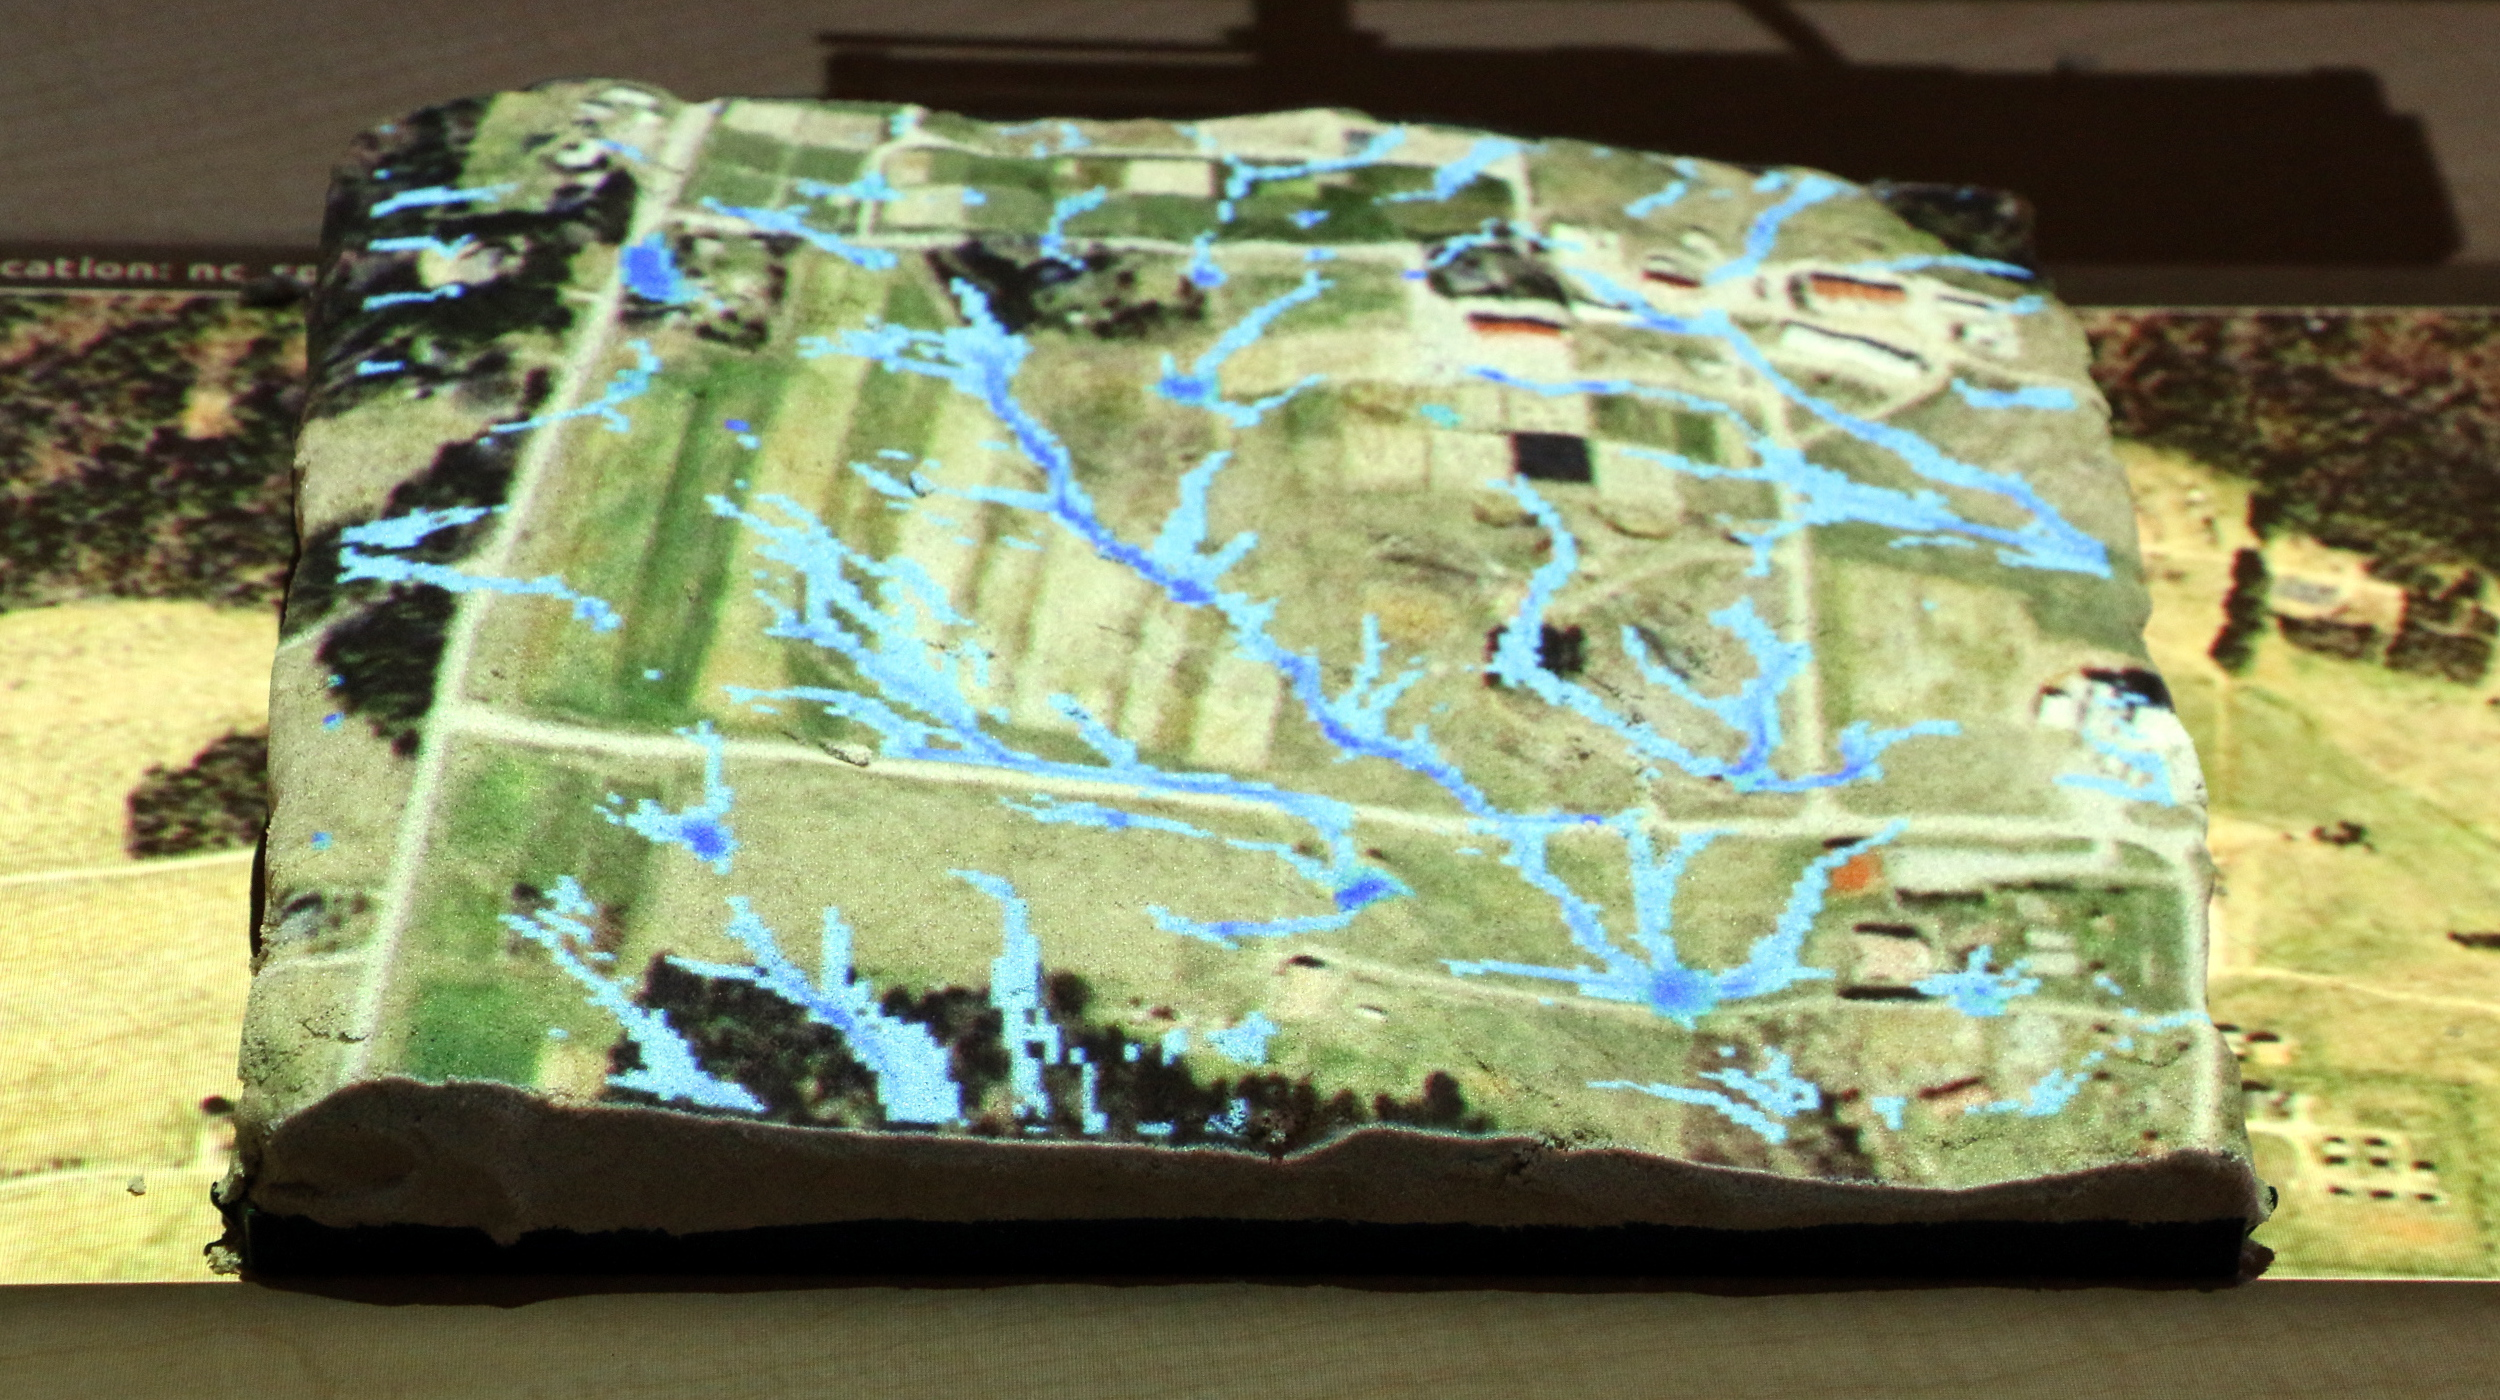
\includegraphics[width=0.32\textwidth]{images/tl_sequence_1.jpg}
		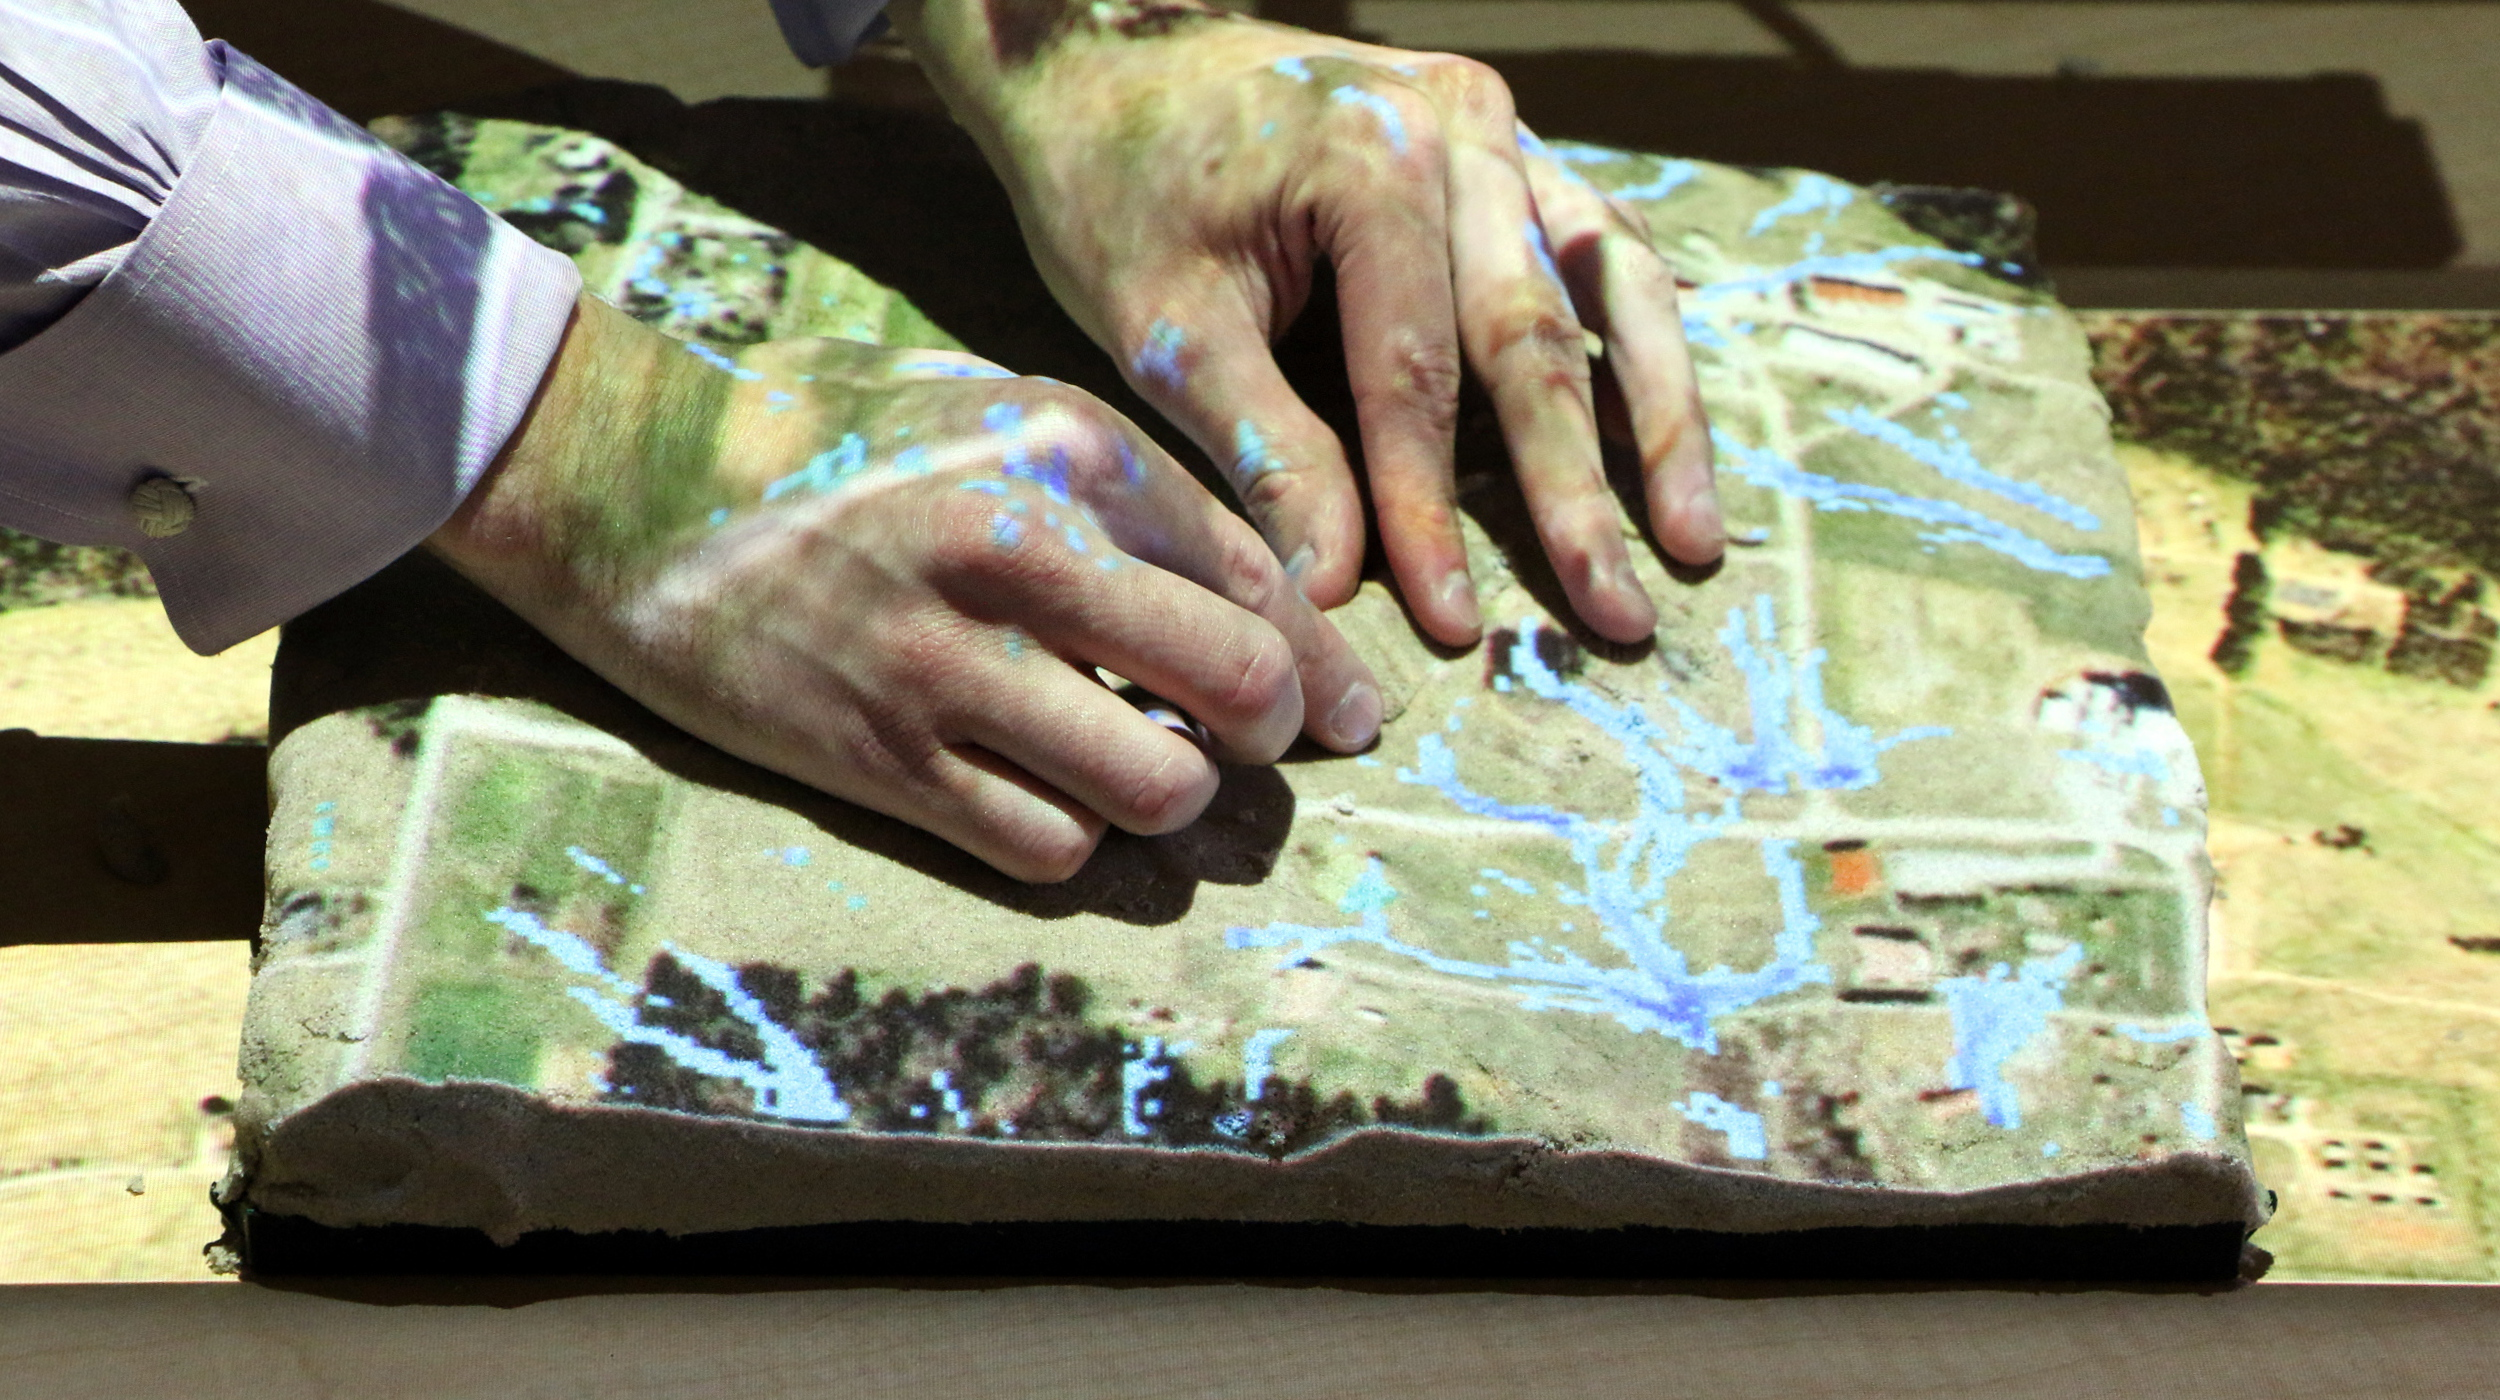
\includegraphics[width=0.49\textwidth]{images/tl_sequence_2.jpg}
		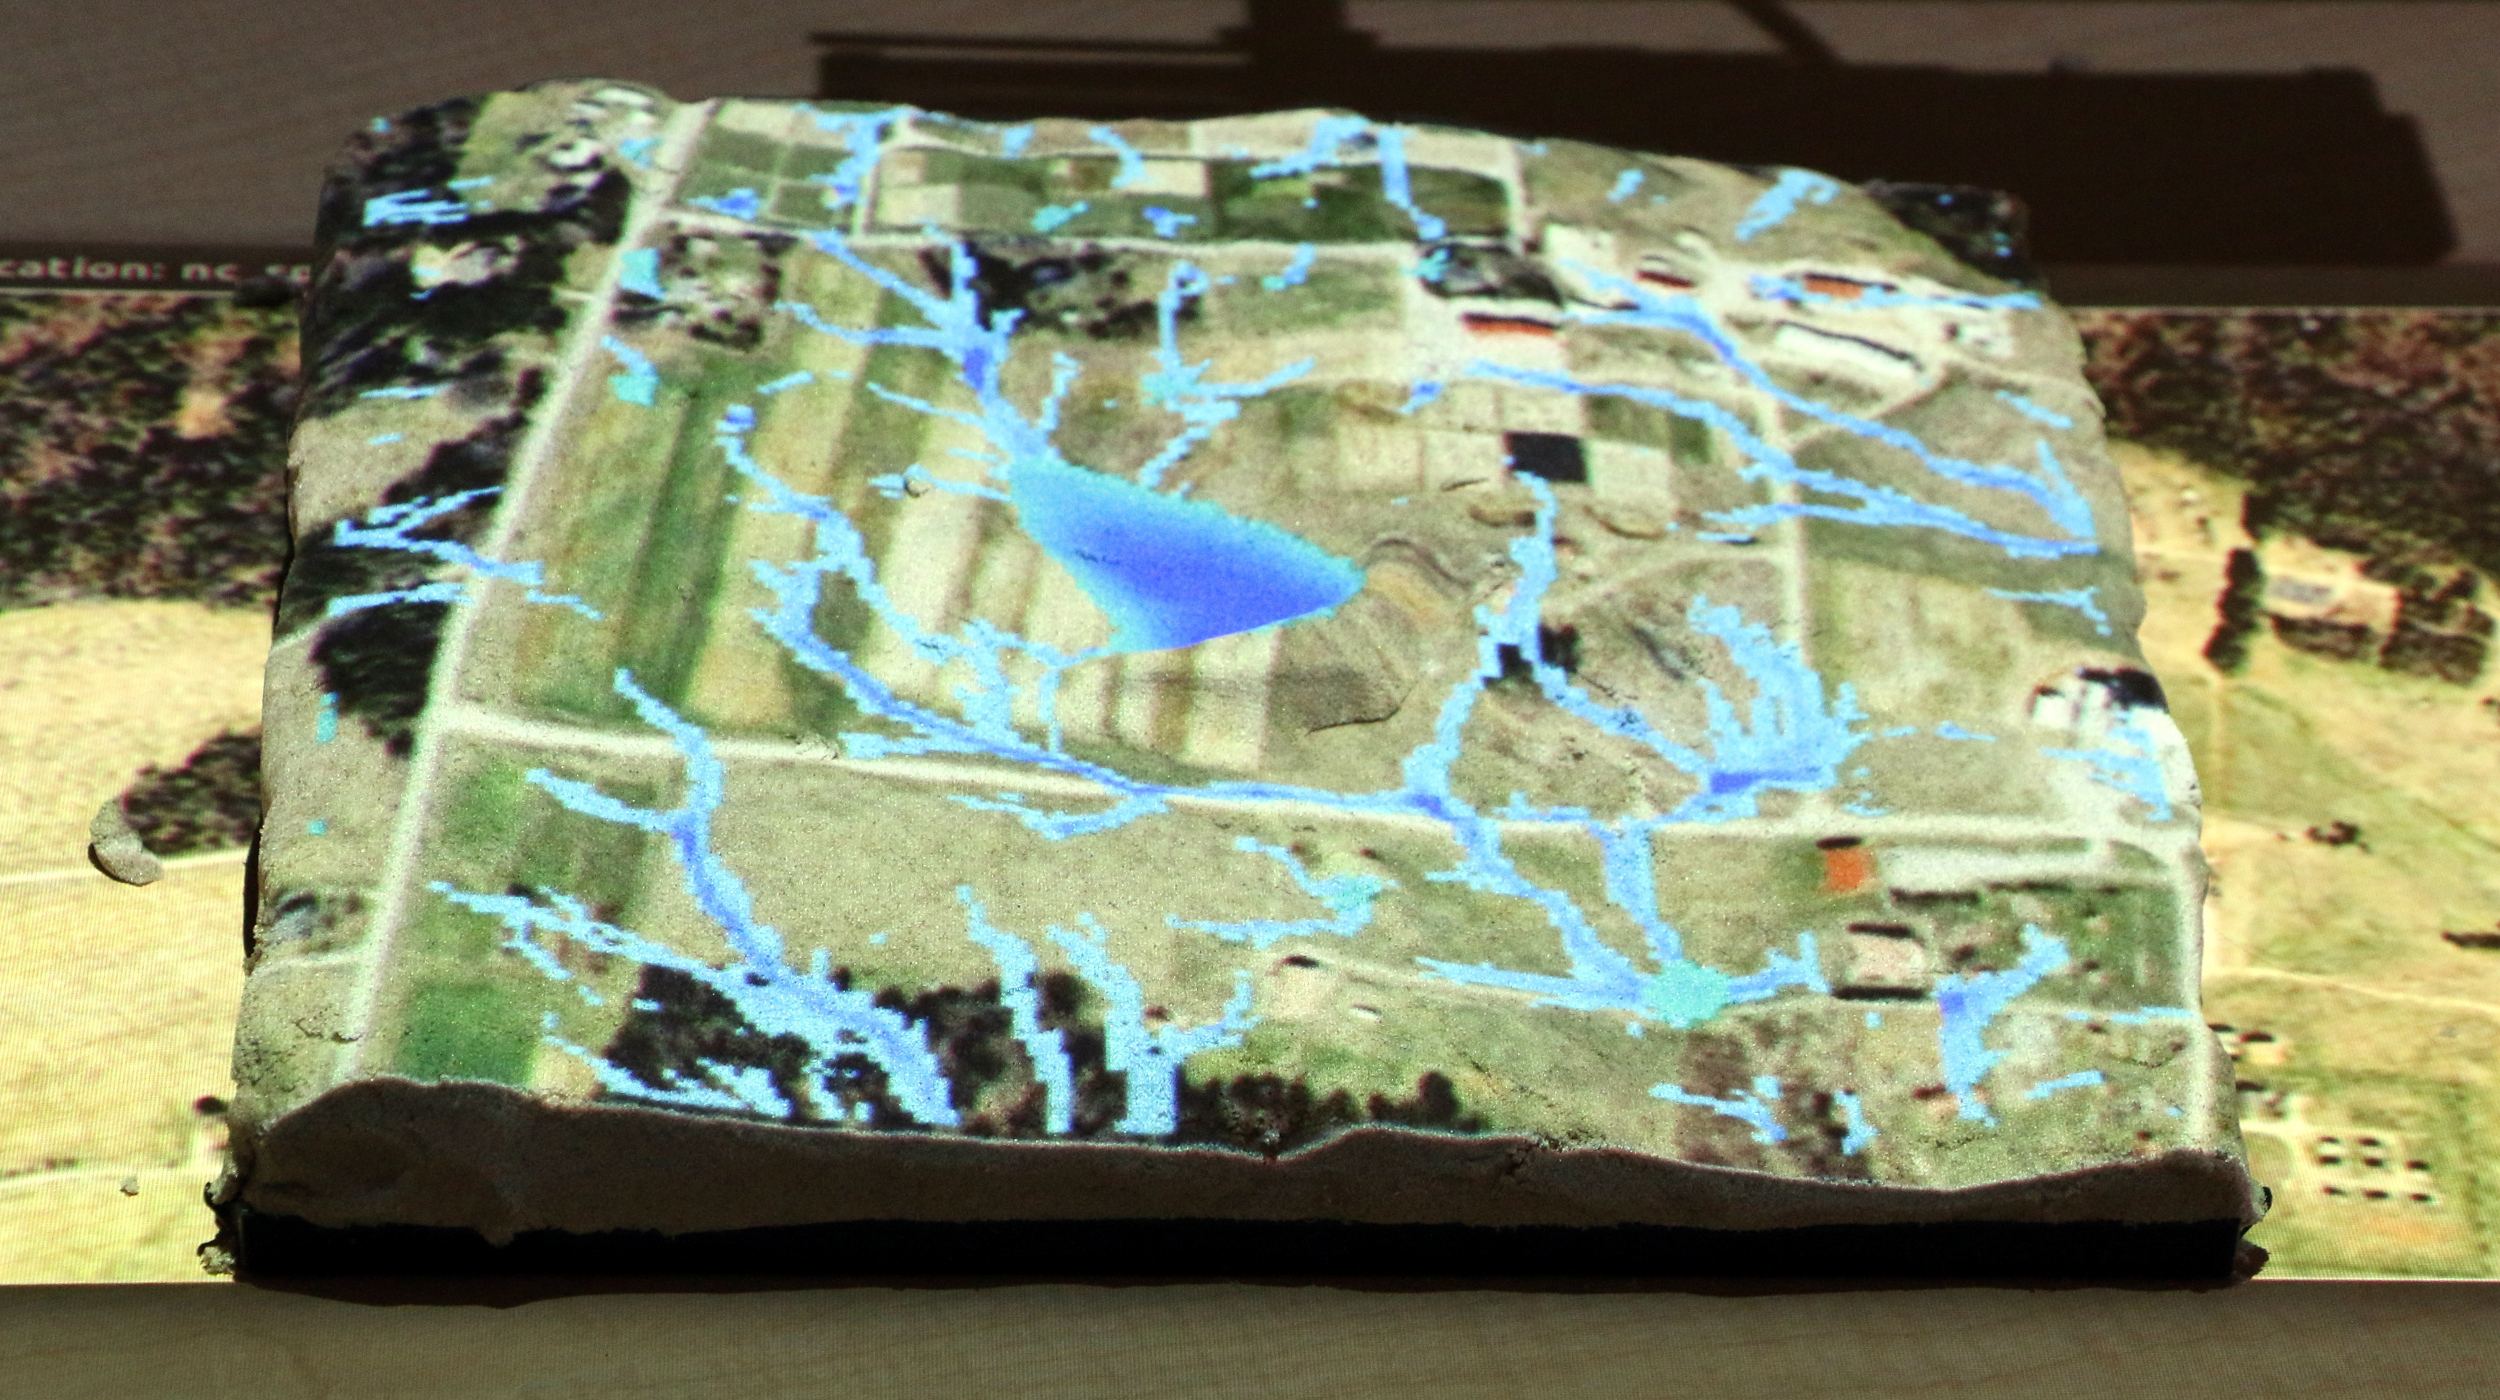
\includegraphics[width=0.49\textwidth]{images/tl_sequence_3.jpg}
	\caption{Tangibly modeling the flow of water with Tangible Landscape}
	\label{fig:tl_flow}
\end{center}
\end{figure*}


% A brief intro to TL
We present Tangible Landscape -- 
a tangible interface for geographic information systems (GIS). 
%
GIS can be used to quantitatively model, analyze, simulate, and visualize 
complex spatial and temporal phenomena 
-- computationally enhancing users' understanding of space. 
%
GIS, however, can be unintuitive and challenging to use. 
%
Unintuitive interactions with GIS can 
frustrate users,
constrain how they think about space,
and add new cognitive burdens
requiring highly developed spatial skills and reasoning. 
%
In order to make GIS more natural and intuitive to use
we have designed a tangible interface for GIS
that physically manifests digital data 
so that users can feel and manipulate it with their bodies (Fig.~\ref{fig:tl_flow}). 
%
We designed Tangible Landscape
so that users can hold a GIS in their hands
and think about 
space and spatial computations 
kinaesthetically with their bodies.
%
Our goal is for users with little or no computer experience 
to be able to intuitively, collaboratively explore spatial data and scientific models and 
rapidly test ideas while learning from computational feedback. 
%
%In order to test, critique, and refine our design
%and advance the study of embodied cognition and tangible interaction 
%we quantitatively analyzed through a series of experiments how 
%Tangible Landscape mediates spatial cognition. 
In a series of experiments we have begun to
quantitatively analyze how 
Tangible Landscape mediates spatial cognition. 
%
We invite other researchers to collaborate 
in this ongoing open source and open science project 
by building Tangible Landscape,
contributing to its development,
developing new applications, 
and studying how it mediates cognition. 

\subsection{Spatial thinking and computation}

Spatial thinking -- `the mental processes of representing, analyzing, and drawing inferences from spatial relations' \cite{Uttal2013} -- is used pervasively in everyday life % at a personal scale 
for tasks such as recognizing things, manipulating things, interacting with others, and way-finding. 
%
Spatial thinking is also used extensively in science, technology, engineering, the arts, and math 
for tasks like 
diagramming concepts, 
visualizing data, % \cite{Ormand2014}
simulating physical processes,
mapping and manipulating molecules,
designing circuits, 
designing buildings, 
shaping sculpture,
and studying topology. 
%
Given the importance of spatial thinking -- personally, academically, and professionally -- 
how can we effectively improve spatial performance, the ability to perform tasks that require spatial thinking? 

% `Spatial thinking is malleable ' \cite{Uttal2013}.

Many spatial tasks can be performed computationally 
enabling us to efficiently store, model, and analyze large sets of spatial data 
and solve complex spatiotemporal problems.
%
In engineering, design, and the arts 
computer-aided design (CAD) and 3D modeling software are used to interactively, computationally model, analyze, and animate complex spatial forms. 
%
In scientific computing spatial patterns and processes can be mathematically modeled, simulated, and optimized. 
%
Geographic information systems for example can be used to computationally store, model, analyze, simulate, and represent geospatial patterns and processes. 
%
The open source 
Geographic Resource Analysis Support System (GRASS) GIS supports 
`geospatial data management and analysis, image processing, graphics and maps production, spatial modeling, and visualization' \cite{GRASS}. 
%\footnote{\url{https://grass.osgeo.org/}} 

Computing mediates and transforms spatial thinking, expanding, but also constraining what is possible.
%
While spatial computing can augment spatial thinking 
-- distributing or offloading cognitive processes through digital computation -- 
the logic of implementation,
the limits of what is computationally possible, 
and the modes of input and output
constrain how we reason. % citations
%
Furthermore, 
when it is difficult to interact with a computer, 
to input commands and parse the resulting output, 
one has to think harder and risks frustration and demotivation. % citations 

Unintuitive modes of human-computer interaction constrain thought and add cognitive and emotional costs. 
%
The paradigmatic modes for interacting with computers today 
-- command line interfaces (CLI) and
graphical user interfaces (GUI)
%including touch interfaces
 -- 
require physical input from devices like keyboards, mice, digitizing pens, and touch screens, but
output %render
data visually as text or graphics. 
%
Theoretically this disconnect between intention, action, and feedback should make interaction less intuitive \cite{Dourish2001,Ishii2008}. 
%
Furthermore, it can also be challenging to parse data that is only presented visually. 
Spatial data -- especially 3D spatial data -- presented graphically can require sophisticated spatial reasoning skills such as mental rotation \cite{Shepard1971}, spatial visualization, and spatial perception \cite{Linn1985} to parse and understand, much less manipulate. 

\subsection{Tangible interaction}
% Introduction to tangible interfaces
Tangible interfaces -- interfaces that couple physical and digital data \cite{Dourish2001} -- 
are designed to physically manifest digital data so that we can cognitively grasp and absorb it,
so that we can think with it rather than about it \cite{Kirsh2013}. 
%
Ishii and Ullmer envisioned that tangible interfaces would  `take advantage of natural physical affordances to achieve a heightened legibility and seamlessness of interaction between people and information' \cite{Ishii1997}. 
%
With a tangible interface both input and output are physical. 
%
Data can be felt as well as seen; data can be directly, physically manipulated, leveraging highly developed motor skills. 
%
Thus intention, action, and feedback should be seamlessly connected 
enabling automatic, subconscious, and intuitive interaction.

% Embodied interaction
Tangible interfaces let users interact with computers while (functionally) thinking with their bodies. 
%
By thinking with their bodies, by embodying cognition 
users may be able to reduce their cognitive loads by
offloading cognitive tasks like 
spatial perception and manipulation 
onto the body and 
physically simulating processes.
%
In embodied cognition higher cognitive processes are grounded in, built upon, and mediated by bodily experiences such kinaesthetic perception and action \cite{Hardy-Vallee2008}. 
%
When people use tools they temporarily, contingently incorporate them into their body schema, feeling the perimeter, weight, and balance of the tool, 
sensing resistance when the tool touches something, 
as if the tool was an extension of the body \cite{Maravita2004}.
%
Because tools can be cognitively gripped and absorbed in users' body schema, tools mediate embodied cognition -- affording new bodily experiences and actions and thus extending users' capacity for thought. 
%
Tangible interfaces are designed to make computation tangible so that it can be cognitively gripped and absorbed, so that computation can be understood with and offloaded onto the body.
%
When tangible interactions are designed to be analogous to everyday, physical tasks 
like unscrewing a bottle top \cite{Kirsh2013}, 
picking up and placing objects, 
or sculpting sand 
users may already understand what to do; 
such interaction should be highly intuitive
drawing on existing cultural knowledge and motor schemas. 

% Tangible interaction and spatial cognition
It can be challenging and cognitively taxing to visually perceive and parse space, to for example visually judge distances and imagine volumetric form.
%
Distance and physical properties like size, shape, volume, weight, hardness, and texture, however, can be automatically and subconsciously assessed kinaesthetically with the body \cite{Jeannerod1997}. 
%
By affording physical feedback tangible interfaces should, therefore, reduce the cognitive load needed to judge and manipulate spatial distances, relationships, patterns, and forms. 
%
Tangible interfaces have been shown to significantly improve spatial performance 
over graphical interfaces \cite{Cuendet2012}.

\begin{figure*}[h!]
\begin{center}
		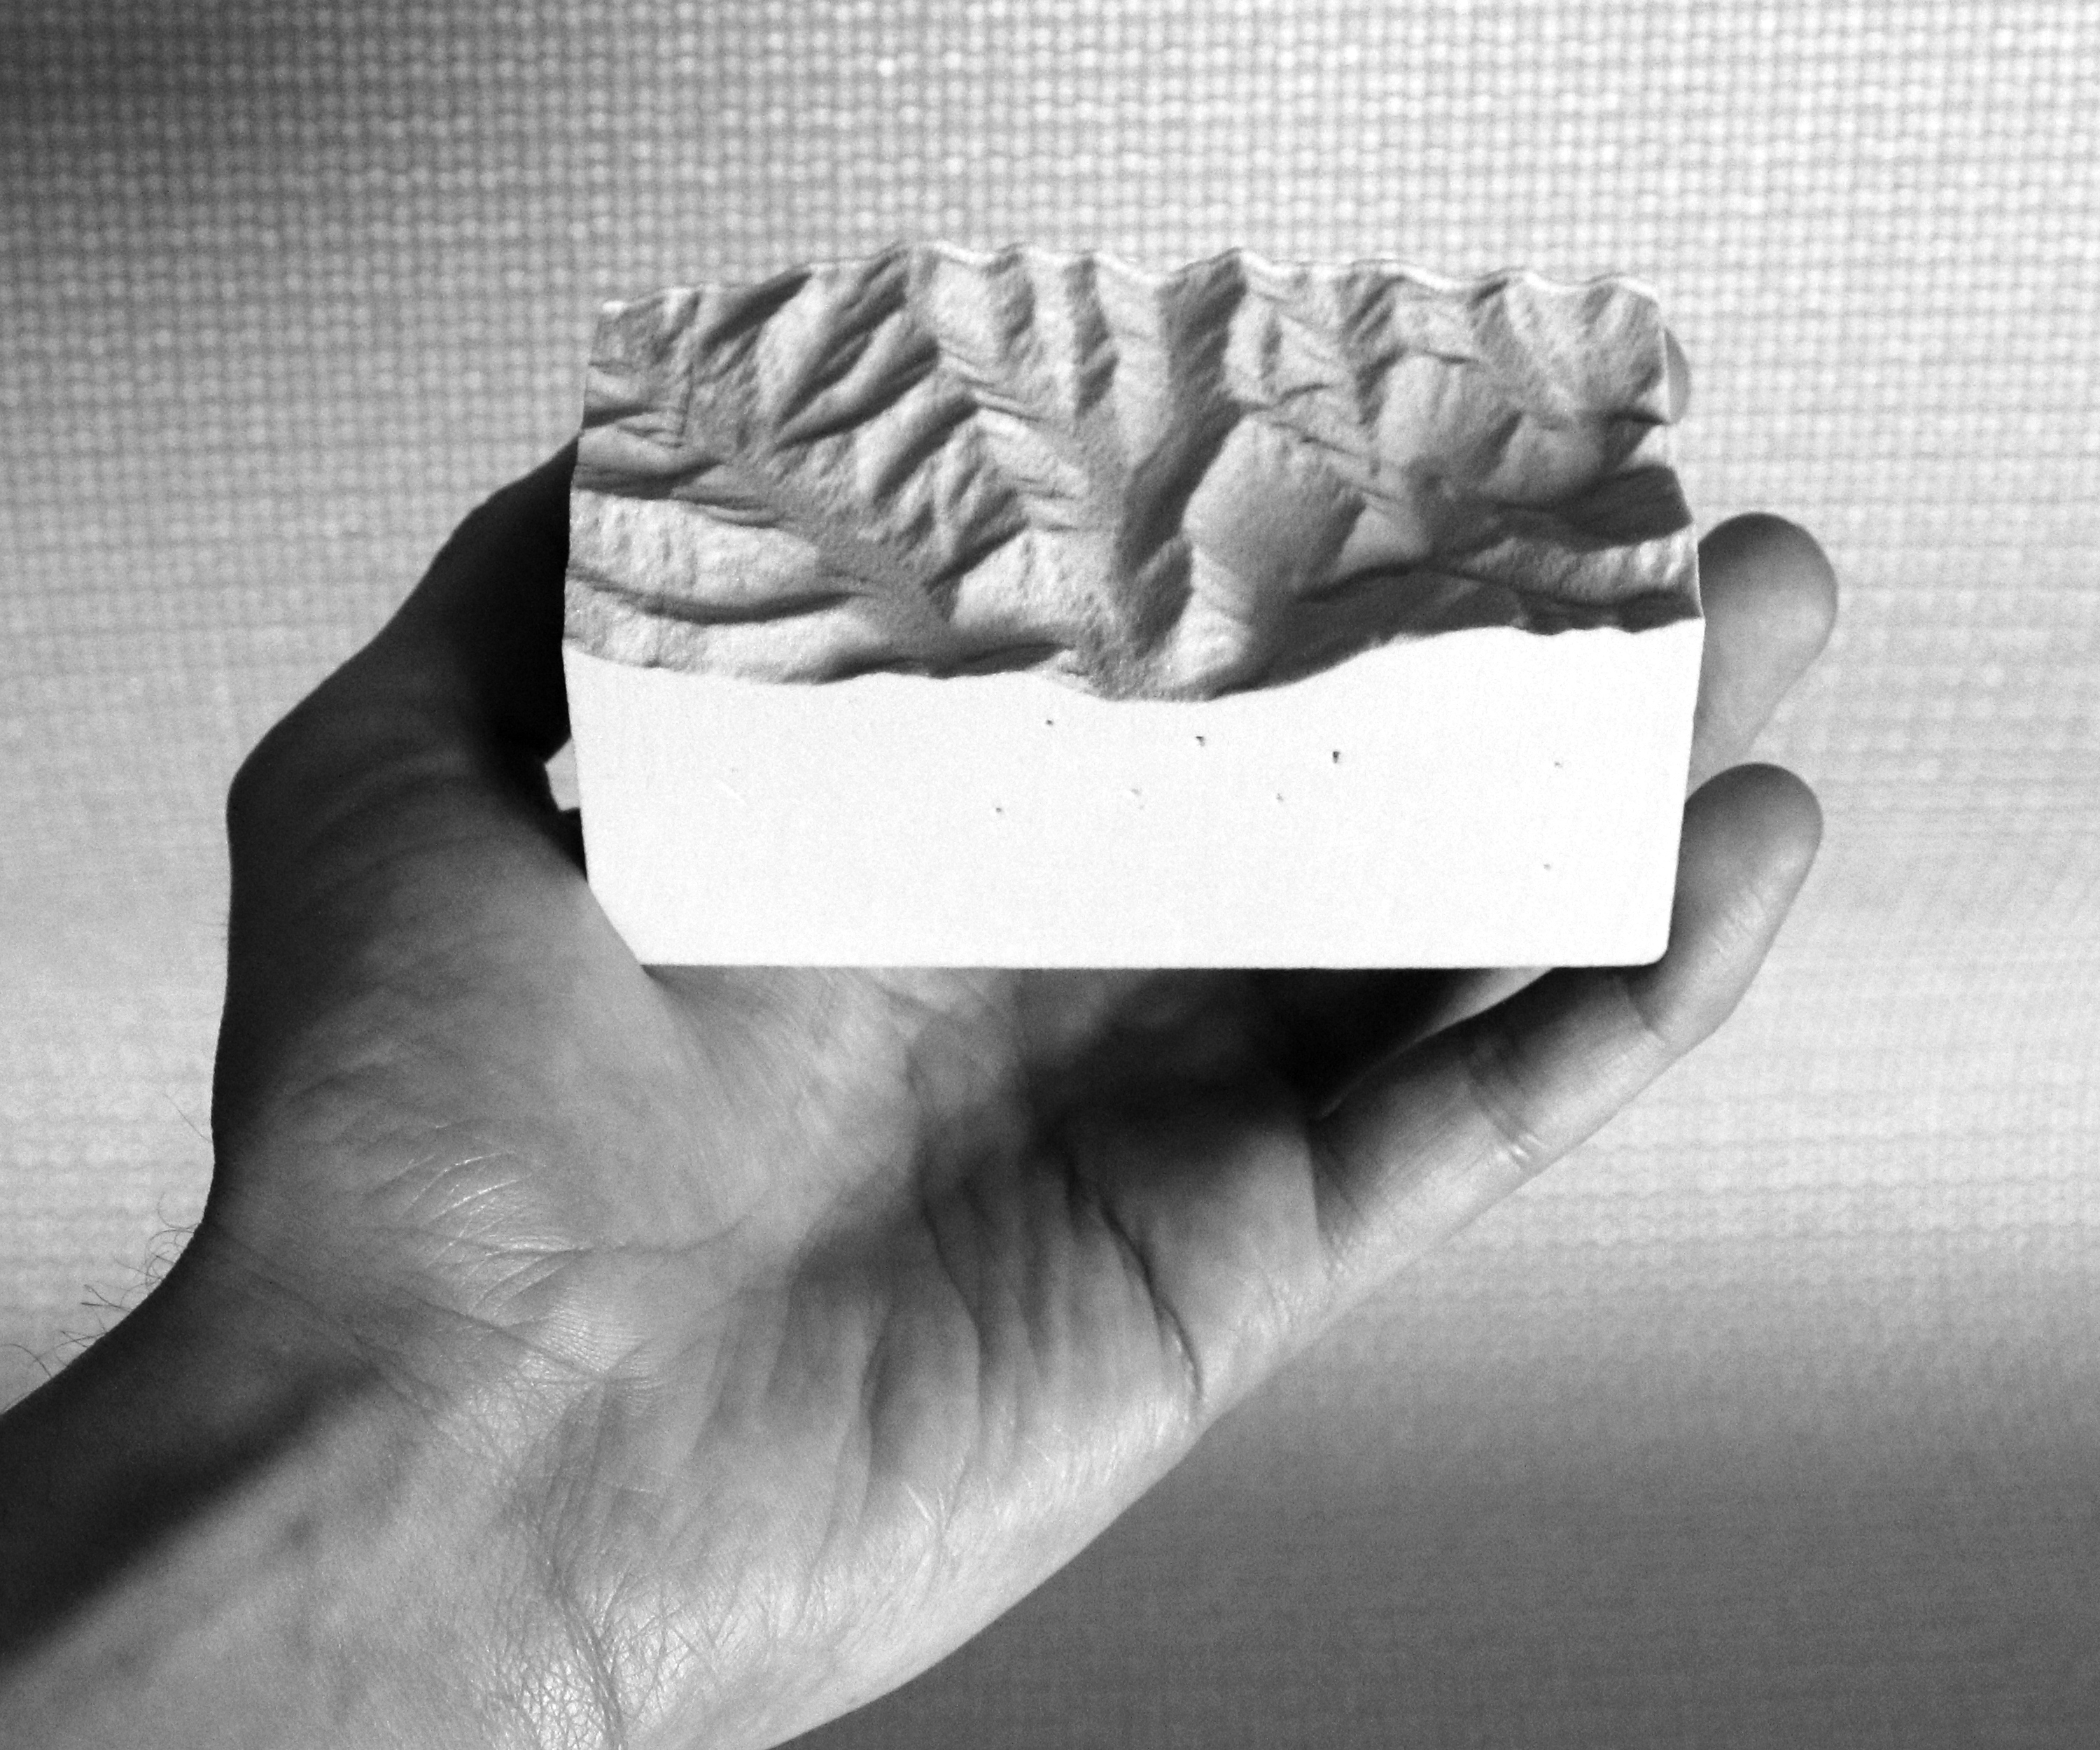
\includegraphics[width=0.49\textwidth]{images/physical_rotation_1.jpg}
		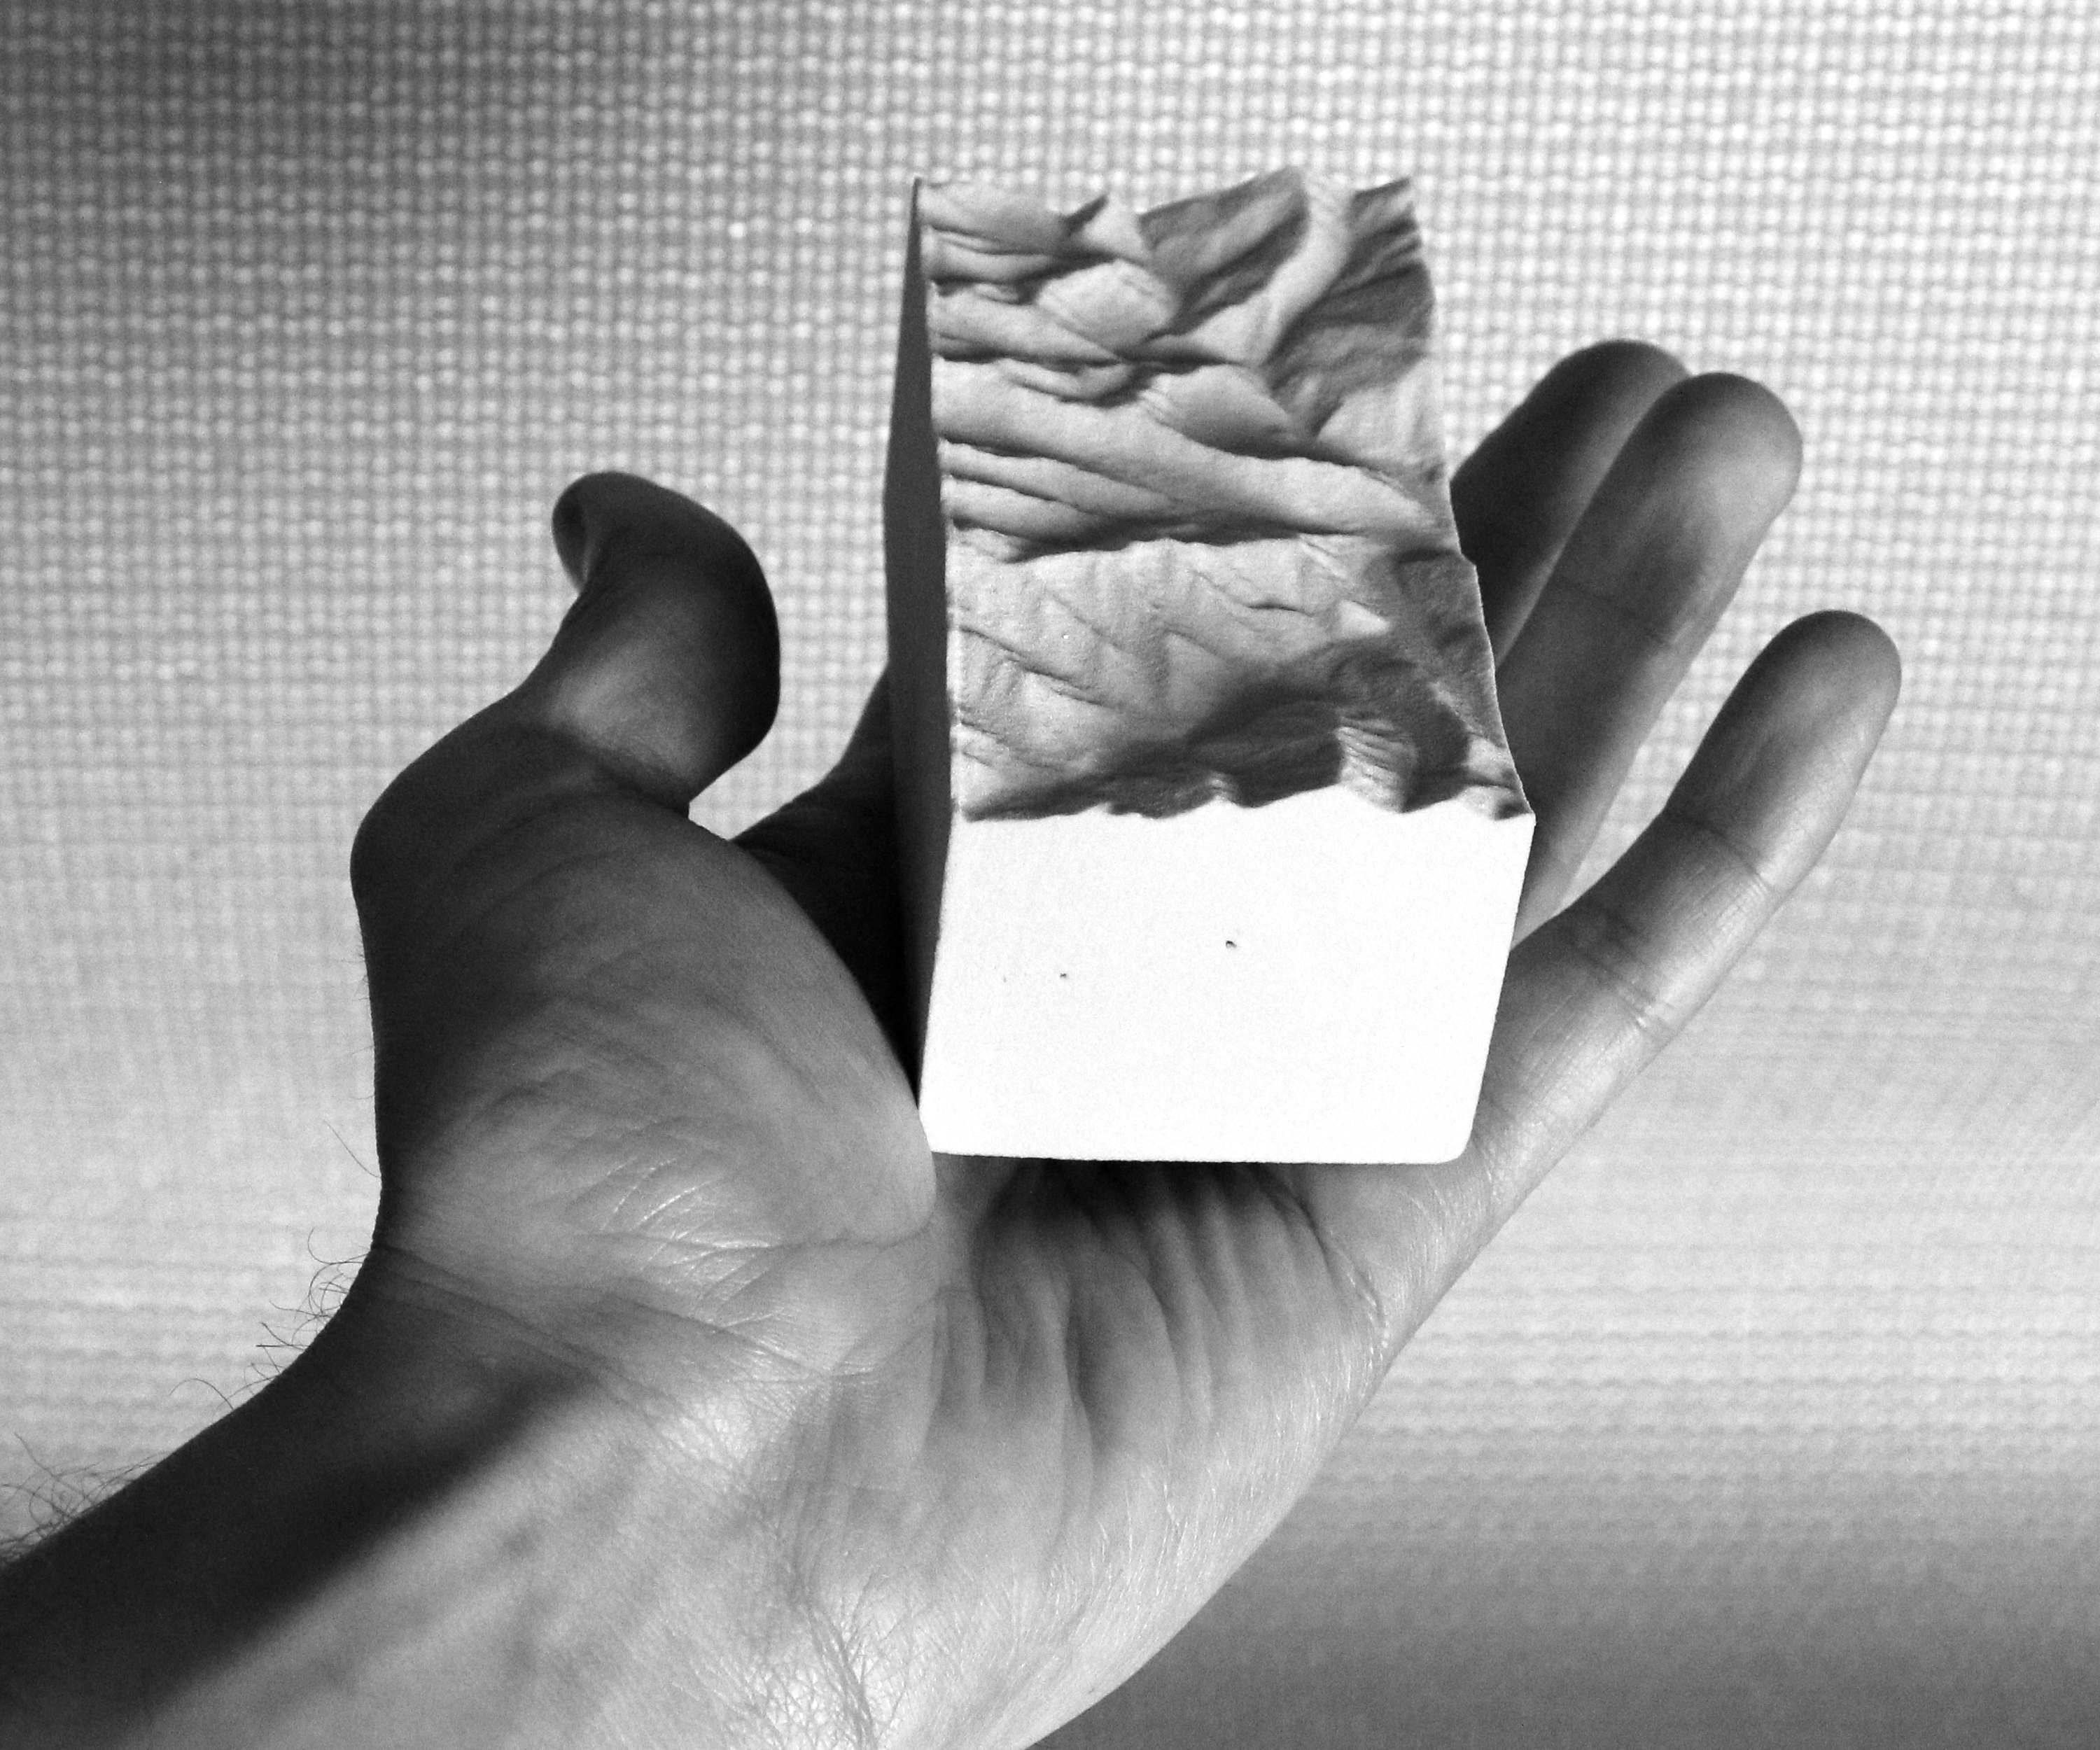
\includegraphics[width=0.49\textwidth]{images/physical_rotation_2.jpg}
	\caption{Physically rotating a topographic model}
	\label{fig:physical_rotation}
\end{center}
\end{figure*}

% Physical simulation
Furthermore, some cognitive processes can be physically simulated, offloading cognitive work onto the body \cite{Kirsh2013}. 
%
Mental models can be abstracted and physically simulated 
through acting, 
sketching, 
or experimental adaptation or transformation. 
%
Kirsh cites the dancers use of marking 
-- a simplified, abstraction of a dance phrase -- 
to learn and practice elements or aspects of the phrase \cite{Kirsh2013}. 
%
% Mental rotation
Mental rotation 
-- a cognitive task commonly used in psychometric tests of spatial ability -- 
can be physically simulated 
simply by grasping the object and rotating it (Fig.~\ref{fig:physical_rotation}).
%
While tasks like spatial visualization and mental rotation are used assess spatial ability
\cite{Uttal2013a,Uttal2013,Ormand2014}, 
space is not just visualized, but also felt.
Space need not be imagined to be transformed. 
%--haptic feedback about space informs subconscious pragmatic representations that rapidly generate action \cite{Jeannerod1997}. 
Mental rotation and spatial visualization, therefore, 
may tell us little about embodied spatial ability. 

% Form finding
Metacognition -- thinking about thinking -- 
can play an important role in embodied spatial performance.
%
Physical simulation guided by metacognitive reflection 
is used in generative, creative processes 
such as sculptural form-finding or gestural sketching. 
%
Professionals like designers develop creative ideas through `reflection-in-action,' 
an iterative, exploratory, metacognitive process 
of framing a problem, ideation or making, and critical reflection \cite{Schon1983}.
This exploratory process may unfold in an instant, 
repeated continually throughout acts such as drawing, sculpting, and modeling. 
%
The architect Frank Gehry for example develops his designs through exploratory form finding with massing models
and by thinking through the movement of gestural drawing
\cite{Gehry2004,Pollack2006}.
%
An ethnography of the Office of Metropolitan Architecture
showed that architects in the firm used exploratory modeling
to develop designs in iterative process
-- exploring form by carving foam massing models with hot-wire cutters, reflecting on each model as they carved, while building up a library of forms \cite{Yaneva2009}.

% Metacognition in tangible interaction
Tangible interfaces enable embodied interaction
-- the kinaesthetic exploration and physical transformation of digital data.
%
By embodying interaction
users can offload 
challenging cognitive tasks 
like sensing form, manipulating form, and imagining new forms 
onto the body
-- freeing up more cognitive resources for  
metacognition. 
%
With more resources for metacognition
users should be better able to parse and learn from computations.
%
With GIS users can computationally offload other types of challenging cognitive tasks 
like analyzing spatial patterns and simulating spatiotemporal processes.
%
Tangible interfaces for GIS should, therefore, enhance users' spatial performance 
by combining these physical and computational affordances.

\subsection{Research questions}

\begin{itemize}
% design
\item How can we design an effective tangible interface for GIS?
% coupling
\item Can coupling a physical and digital model of topography improve spatial performance?
% analytics
\item How do different geospatial analytics mediate users' spatial performance when using a tangible interface for GIS?
\end{itemize}

\section{Methodology}
\subsection{Tangible Landscape}

\paragraph{Concept}
%
Tangible interfaces for GIS 
should ease the cognitive burden of 
visualizing, interacting with, reasoning about space
by giving spatial data an interactive, physical form 
that users can cognitively grasp and kinaesthetically explore. 
%
Tangible Landscape -- a tangible user interface for GRASS GIS --
couples a physical and digital model of a landscape through a continuous cycle of 3D scanning, geospatial modeling, and projection
so that users can intuitively interact with the modeled landscape in near real-time.
%
Conceptually Tangible Landscape physically manifests geospatial data 
so that users can hold a GIS in their hands -- 
so that they can, for example, feel the shape of the earth, sculpt its topography, and direct the flow of water with their hands.
%
It enables users to 3D sketch -- 
to naturally model forms such as topography, 
draw points and polygons, 
and interact with simulated physical processes -- 
in a rapid, iterative process 
of observation, hypothesis generation and testing, and inference. 
%
Tangible Landscape is meant to fluidly, seamlessly combine
computational science with exploratory modes of creative thinking.

\paragraph{Evolution}
%
Tangible Landscape evolved from 
Illuminating Clay \cite{Piper2002a} and 
the Tangible Geospatial Modeling System (TanGeoMS) \cite{Tateosian2010}. 
%
% Illuminating Clay
Illuminating Clay coupled a clay model and digital model of landscape 
through a cycle of laser scanning, spatial modeling, and projection.
%
By enriching physical models of urban spaces and landscapes 
with spatial analyses  
such as 
elevation, aspect, slope, cast shadow, profile, curvature, 
viewsheds, solar irradiation, and water direction
it enabled
intuitive form-finding, 
streamlined analog and digital workflows, 
and enabled multiple users to simultaneously interact in a natural way \cite{Ratti2004}. 
%
Illuminating Clay had a very limited library of custom implemented spatial analyses. 
%
Since many of analyses were adapted 
from the open source GRASS GIS project \cite{Piper2002a} 
there was a call for closer integration with GRASS GIS 
in order to draw on its extensive libraries 
for spatial computation \cite{Piper2002b}. 
%
The effort to couple a physical landscape model with GRASS GIS \cite{Mitasova2006} 
led to the development of 
TanGeoMS \cite{Tateosian2010}.
%and then Tangible Landscape  \cite{Petrasova2014,Petrasova2015}.

% Tangible Geospatial Modeling System
TanGeoMS coupled a physical model and GIS model of a landscape 
through a cycle of laser scanning, geospatial computation in GRASS GIS, and projection
giving developers and users assess to 
%drawing on 
a sophisticated library for 
spatial modeling, simulation, visualization, databasing.
%
It enriched freeform hand modeling with geospatial simulations like diffusive water flow and erosion-deposition 
so that users could easily explore how 
changes in topographic form affect landscape processes. 

% Augmented Reality Sandbox
Tangible Landscape -- the next generation of this system -- was inspired by
the open source Augmented Reality Sandbox \cite{Kreylos2012}
which couples a sandbox with a digital model of a landscape 
through a real-time cycle of 3D scanning with a Kinect sensor, spatial modeling and simulation, and projection.
%
% TL
While TanGeoMS used an expensive terrestrial lidar scanner for 3D scanning \cite{Tateosian2010}, 
Tangible Landscape uses a low-cost 3D sensor like the Kinect 
for real-time depth and color sensing. 
%
The \nth{1} generation of Tangible Landscape \cite{Petrasova2014} 
used the \nth{1} generation Kinect with structured light sensing \cite{Smisek2011}, 
while the \nth{2}  \cite{Petrasova2015} and \nth{3} generations of Tangible Landscape 
used the \nth{2} generation Kinect with time-of-flight sensing \cite{Bamji2015} . 

% REVIEW OF RESEARCH ON SIMILAR SYSTEMS
% see ARL Sand Table lit review
% as a table


\paragraph{Design}
Tangible Landscape was designed to let users naturally explore 
spatial data, models, and simulations in an engaging, playful way
by 3D sketching (Fig.~\ref{fig:subsurface}).
%
As users sculpt the physical model
the model is 3D scanned as a point cloud, georeferenced, imported into GIS, 
and either binned or interpolated as a digital elevation model. 
The digital elevation model is used to compute 
geospatial analyses, models, and simulations, 
which are then projected back onto the physical model 
-- all in near real-time (Fig.~\ref{fig:system_schema}). 
%
This enables users to tangibly interact with digital models and simulations
either by shaping topography with their hands or
by placing markers that are identified using object and color recognition.
%
Users can also for example use a laser pointer to draw polylines or polygons
that will be detected based on light intensity.
%
As the digital models and simulations update
the results are projected back onto the model for users to see. 

Because the model is continually scanned
users' hands will be digitized as they sculpt or place objects. 
%
Scanning users' hands as topography can be distracting; 
it also, however, helps users understand how the system works
-- by seeing how direct interaction is --
and encourages play. 
Users can, for example, cup their hands over the model 
and see them fill with simulated water. 

\begin{figure}[h!]
\begin{center}
		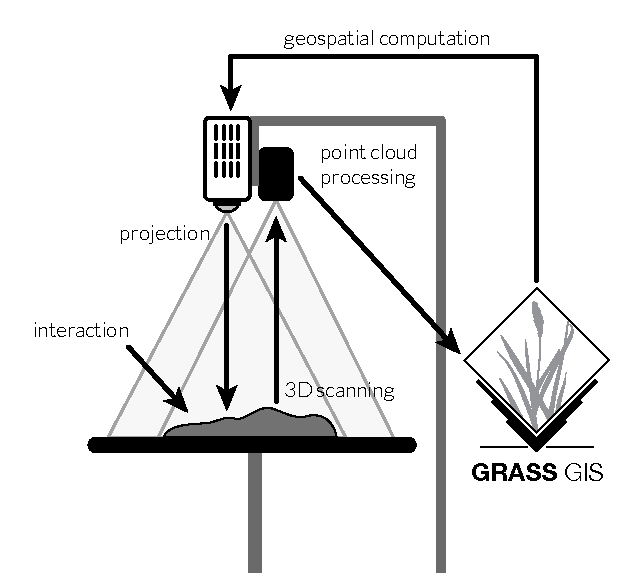
\includegraphics{images/system_schema.pdf}
	\caption{How Tangible Landscape works: a near real-time feedback cycle of interaction, 3D scanning, point cloud processing, geospatial computation, and projection}
	\label{fig:system_schema}
\end{center}
\end{figure}

\begin{figure*}[h!]
\begin{center}
		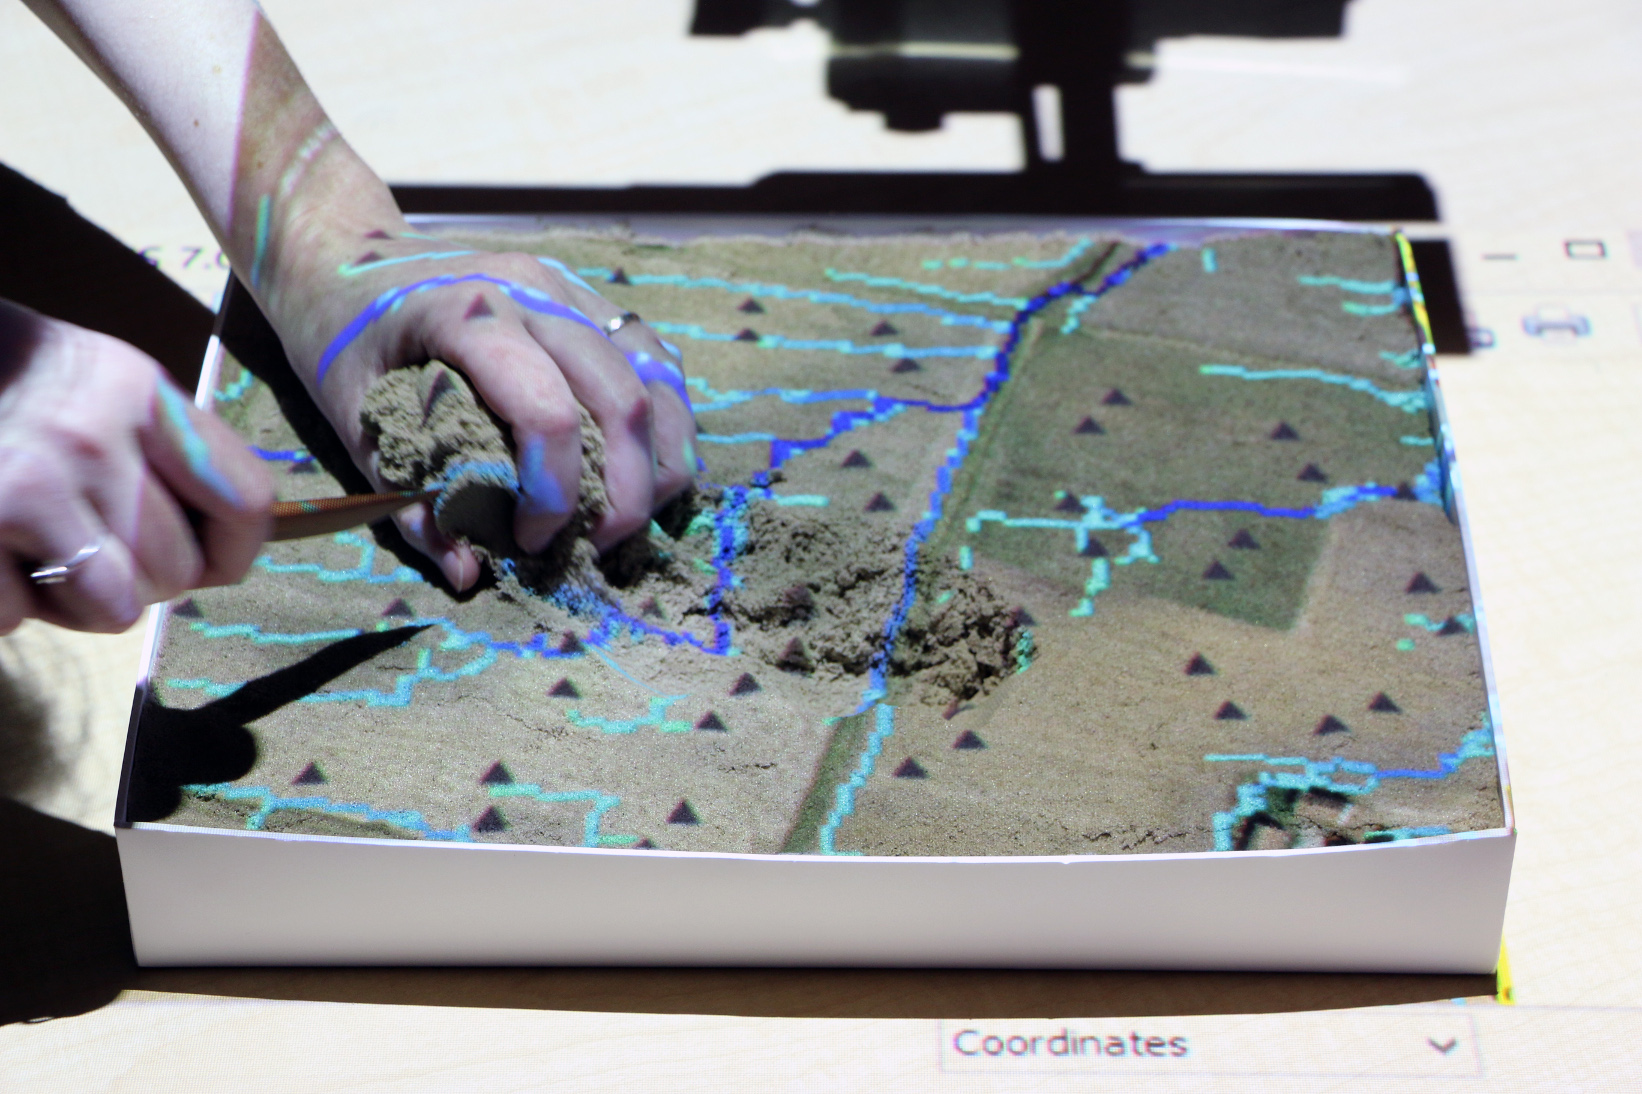
\includegraphics[height=70px]{images/subsurface_1.jpg}
		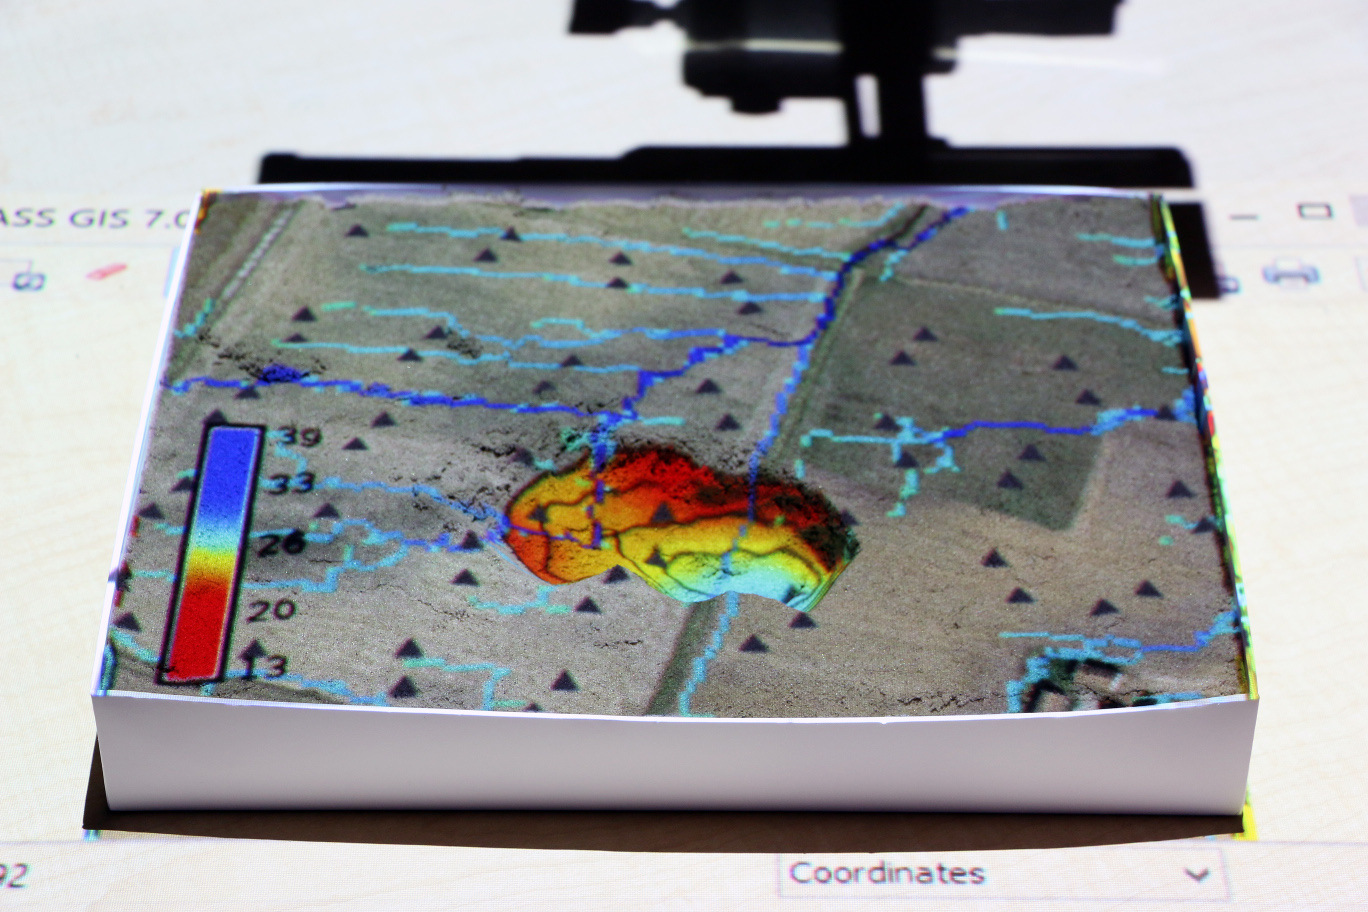
\includegraphics[height=70px]{images/subsurface_2.jpg}
		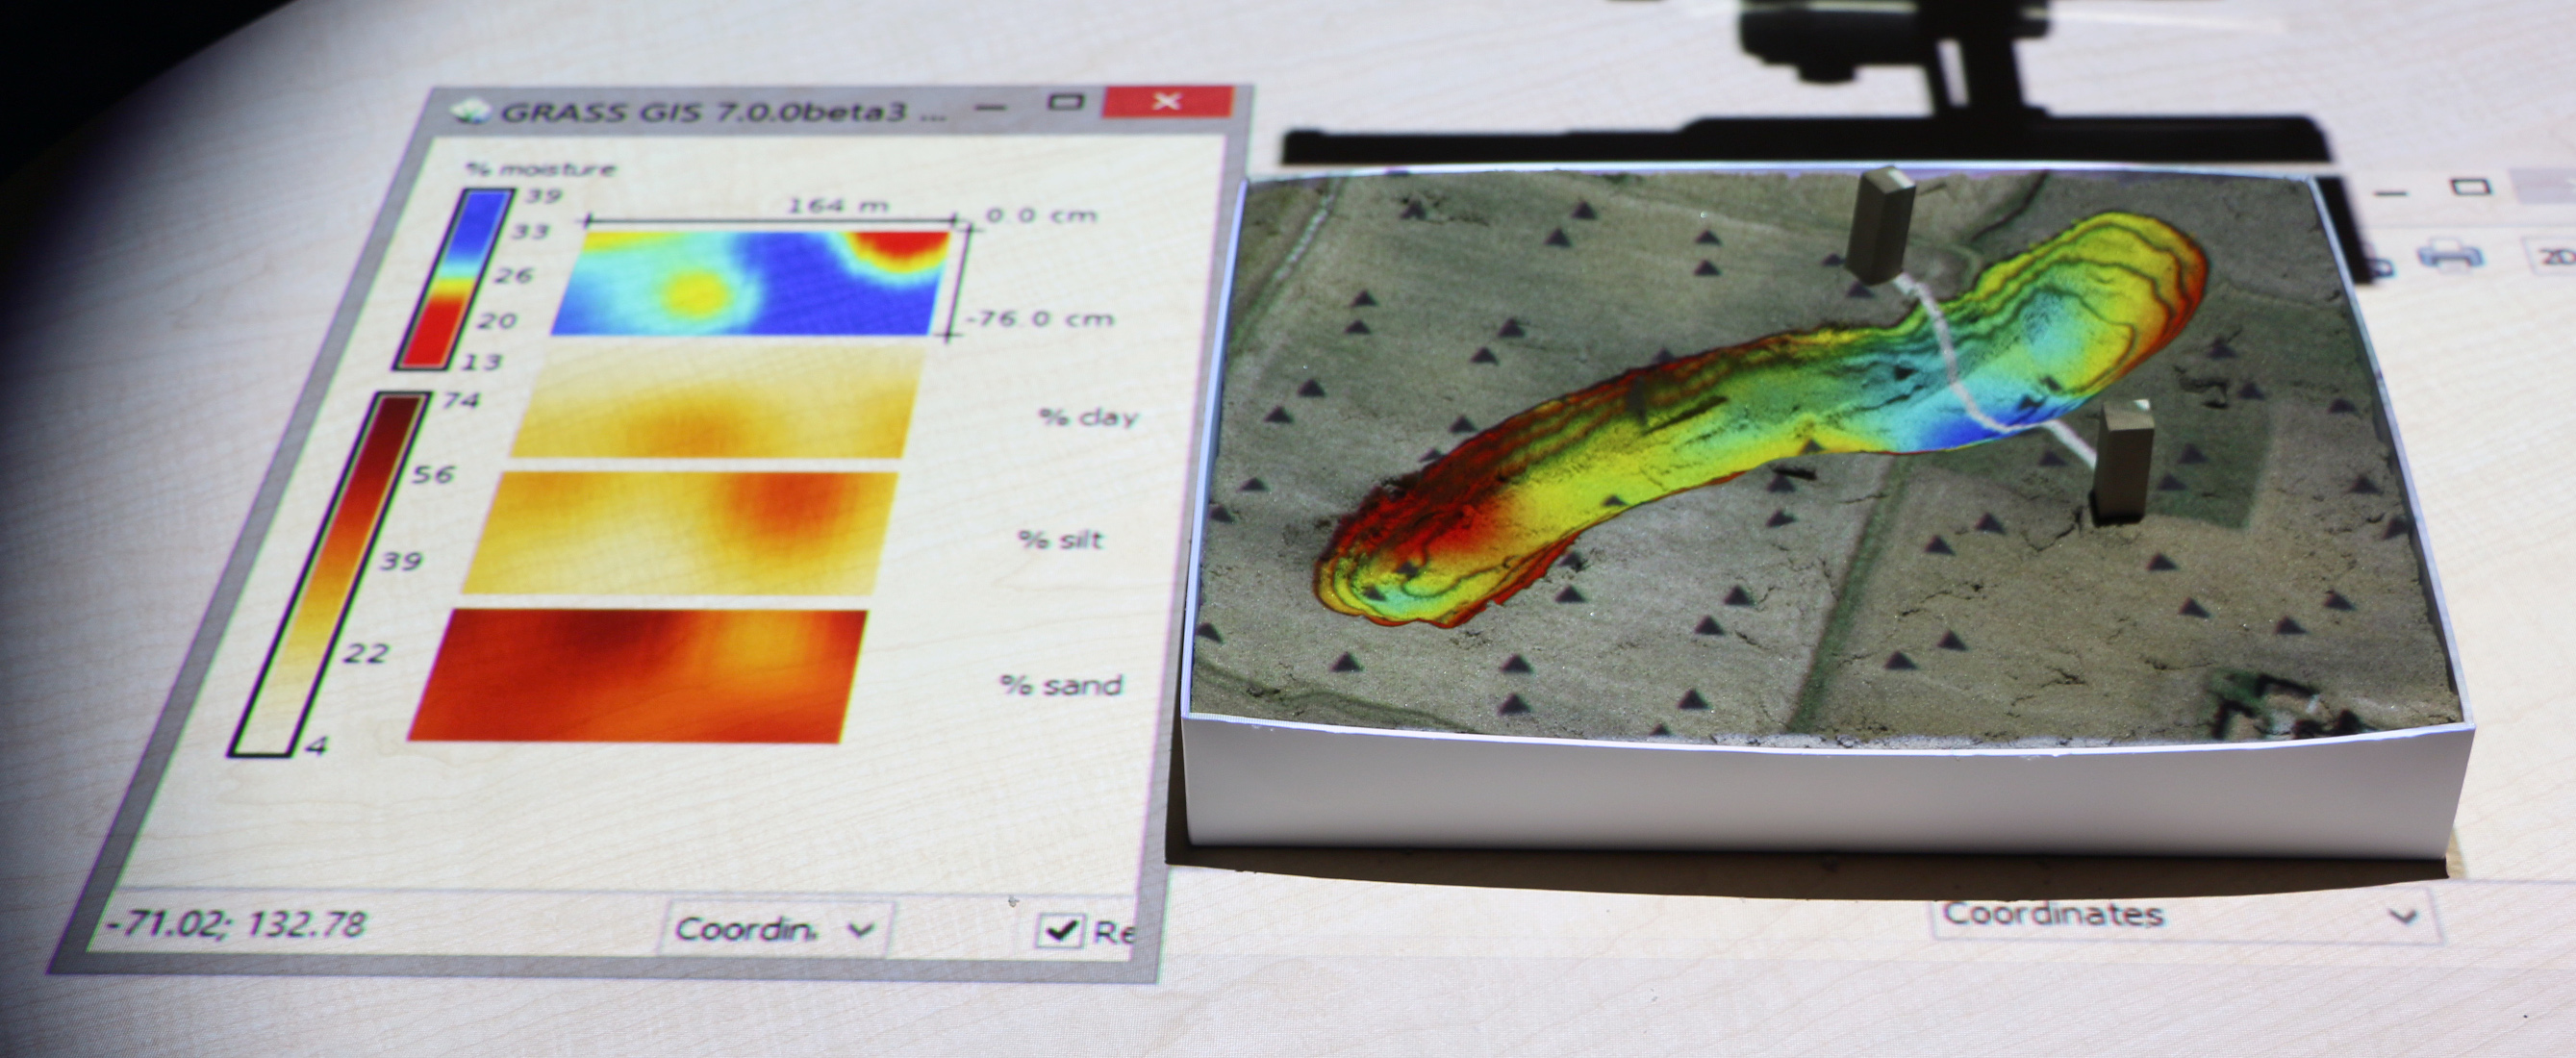
\includegraphics[height=70px]{images/subsurface_3.jpg}
	\caption{Naturally exploring subsurface soil moisture and soil types with Tangible Landscape}
	\label{fig:subsurface}
\end{center}
\end{figure*}

\paragraph{Implementation}
Tangible Landscape has been implemented as a set of components 
-- the r.in.kinect add-on module 
\footnote{\url{https://github.com/ncsu-osgeorel/r.in.kinect}}
and the grass-tangible-landscape plugin 
\footnote{\url{https://github.com/ncsu-osgeorel/grass-tangible-landscape}} --
for the active development version of GRASS GIS. 
%
The r.in.kinect add-on module imports point cloud data from the \nth{2} generation Kinect into GRASS GIS as raster or vector maps. 
It has been implemented as a separate component so that it can easily be used for other applications.
%
The grass-tangible-landscape plugin provides 
utilities, a library of analyses, and a GUI dialog for tangible interaction in GRASS GIS.
%
Users can develop new analyses for Tangible Landscape 
using the GRASS GIS Python Scripting Library.  %GRASS GIS Python API
%
Since many tasks in GIS are not appropriate for tangible interaction
Tangible Landscape was designed to supplement, 
not replace GRASS GIS's GUI, CLI, and scripting API. 

Tangible Landscape currently runs on Linux and Mac OSX 
with an unsupported branch for Windows. 
%
Dependencies include the Point Cloud Library, OpenKinect's libfreenect2, 
OpenCV,  watchdog, and GRASS GIS.

\paragraph{Fabrication}
We typically use familiar, everyday materials 
-- like sand and wooden blocks -- 
for modeling with Tangible Landscape. 
%
Interactions -- sculpting sand and moving wooden blocks -- 
are analogous to everyday tasks
so users should subconsciously know what to do and how to do it, 
leveraging existing sensorimotor schemas. 
%
The materiality -- the feel, look, and physics -- of the media matters. 
The choice of material can afford different interactions
and mediate meaning, emotion, and motivation. 
%
We typically use a polymer-enriched sand for the physical terrain model
so that users can easily sculpt forms in a deformable medium 
that will hold its shape, has good plasticity, and has a familiar feel and aesthetic. 
%
%Polymer-enriched sand can easily be cast in molds and will be hold its form 
%so we often use computer numeric control (CNC) machined or 3D printed molds to
%cast the sand into precise models (Fig.~\ref{fig:casting}.
%
Digital fabrication technologies 
like computer numeric control (CNC) manufacturing and 3D printing
can be used to create molds for casting polymer-enriched sand 
into precise yet deformable models (Fig.~\ref{fig:casting}. 
%
Cast sand models can precisely represent complex forms 
that are challenging to model by hand 
and can easily be re-cast after use.

Tangible Landscape can be also be used as a modeling aid for sculpting.
%
Static projections or dynamic analytics like differencing or water flow 
can be used as guides for hand sculpting terrain models. 
%
Users can project their target digital elevation model and contours 
over their polymeric sand model as a static guide for sculpting. 
%
Tangible Landscape can also dynamically compute the difference -- i.e.\ cut and fill --
between the scanned model that has been sculpted and the target digital elevation model. 
%
The difference can provide a real-time guide 
where to add or remove sand in order to match the target digital elevation model. 
%
% Vertically rescale and translate the scanned raster to match the original DEM using the module r.regression.line.

\begin{figure*}[h!]
\begin{center}
		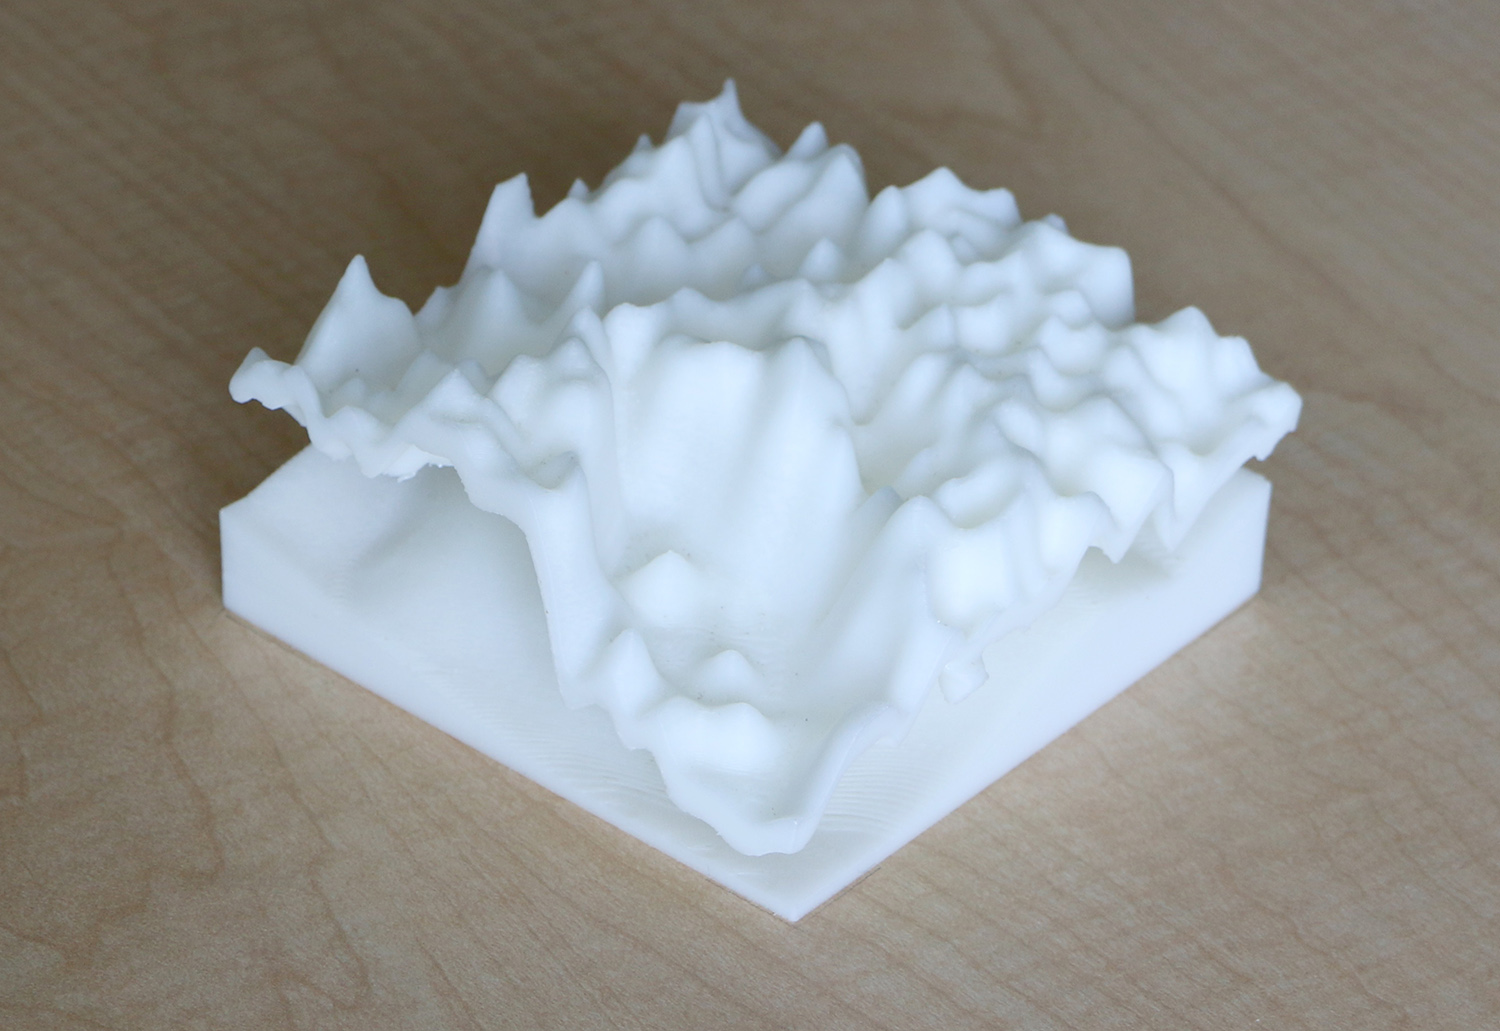
\includegraphics[width=0.3\textwidth]{images/3d_print_1.jpg}
		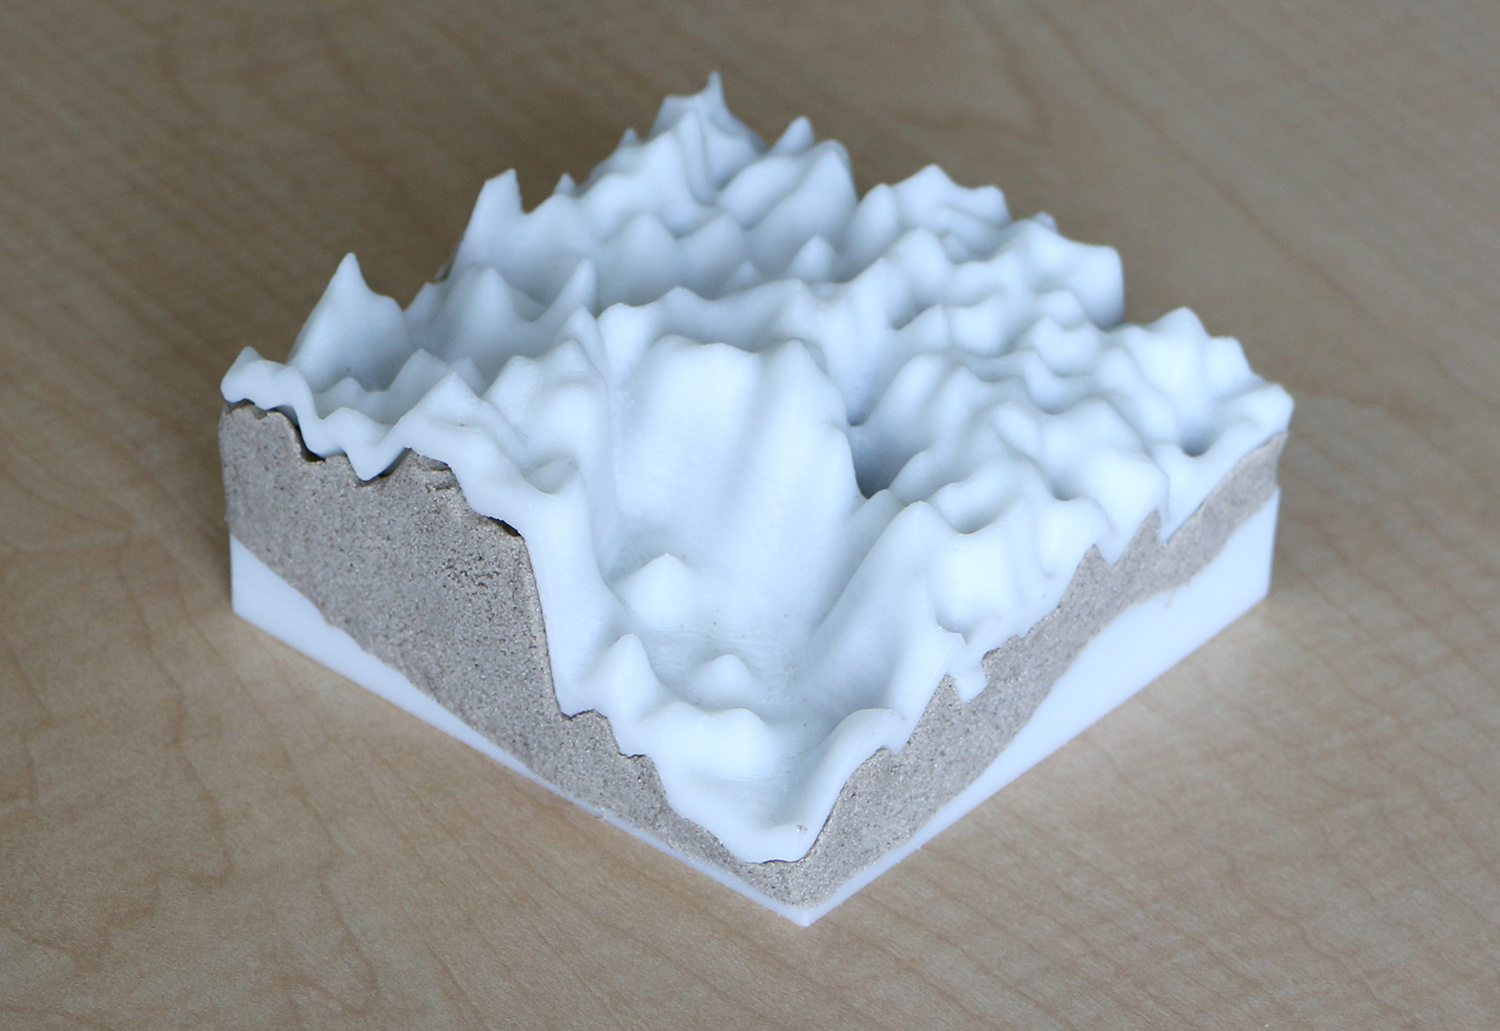
\includegraphics[width=0.3\textwidth]{images/3d_print_2.jpg}
		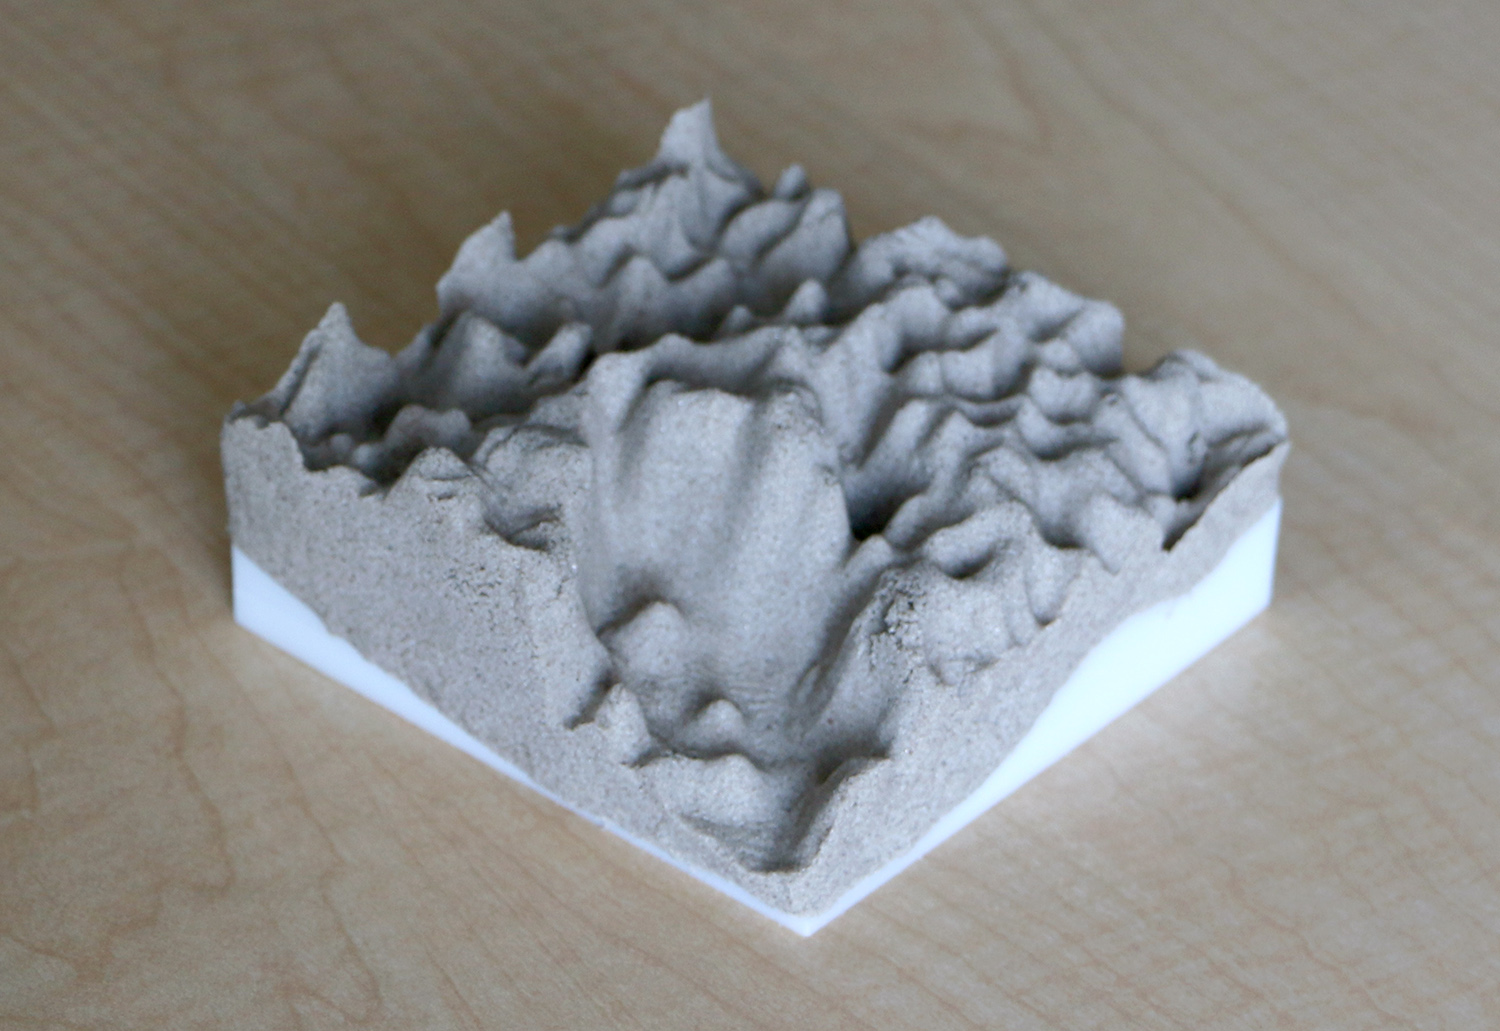
\includegraphics[width=0.3\textwidth]{images/3d_print_3.jpg}
	\caption{Casting polymeric sand with 3D printed molds}
	\label{fig:casting}
\end{center}
\end{figure*}

% Difference figure <----------------------- ADD

% Applications
\paragraph{Applications}
Using GRASS GIS's extensive libraries for geospatial modeling, analysis, and simulation 
we have developed a wide range of applications for Tangible Landscape.
%for disciplines including education, ecology, geomorphology, landscape architecture, urban planning, civil engineering, and disaster management. 
%
Design and planning applications include
grading, cut and fill analysis, stormwater management, erosion control, 
trail planning, viewshed analysis, and the assessment of solar potential. 
%
Scientific applications include
subsurface visualization, disease management, and invasive species management.
%
Disaster management applications include 
flood control, wildfire management, and coastal change and adaptation. 
%
Educational applications include
spatial training and serious gaming.

%\begin{figure*}[h!]
%\begin{center}
%		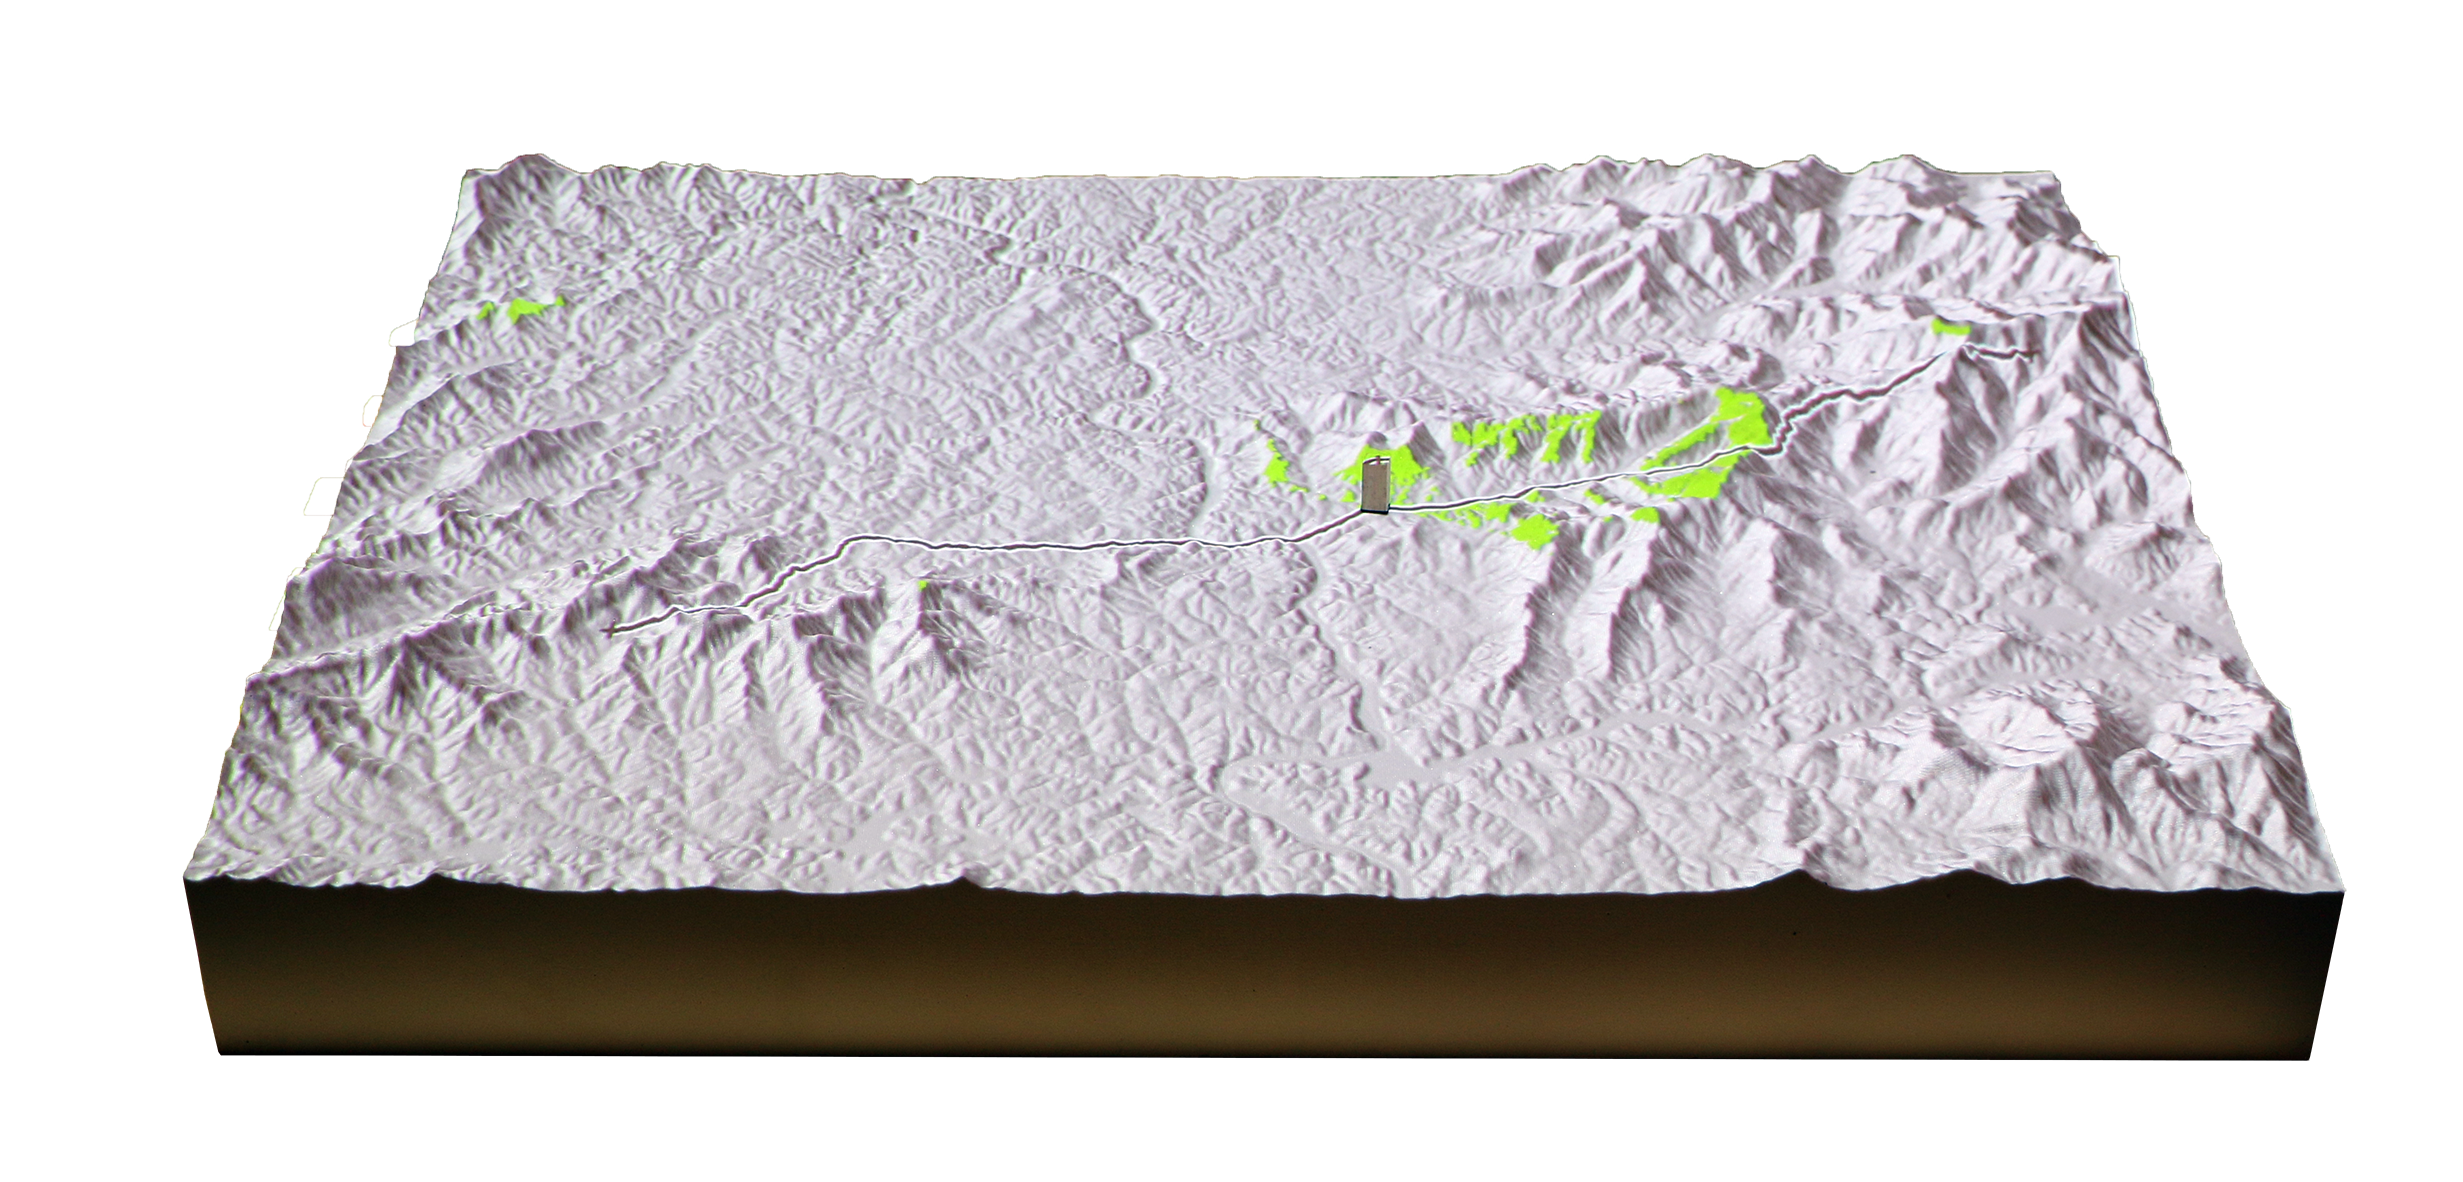
\includegraphics[width=\textwidth]{images/walking_route_view.png}
%	\caption{...}
%	\label{fig:applications}
%\end{center}
%\end{figure*}


\subsection{Coupling experiment}
We conducted an experiment to study how coupling digital and physical models of topography mediates spatial performance. 
%
In this experiment % x 
participants tried to accurately model a given study landscape 
digitally, by hand, and with Tangible Landscape. 

% study landscape
\paragraph{Study landscape}
We used a region of Lake Raleigh Woods in Raleigh, North Carolina 
as the study landscape for this experiment. 
%
We used a real landscape because computer generated landscapes 
often look surreal and may lack distinct landforms and clearly defined streams. 
%
We selected a region with distinctive, 
clearly defined landforms -- a valley, flanked by ridges, sloping towards the lake.
%(see Fig.~\ref{fig:study_area}). 
%
The digital elevation model for this region was derived from a 2013 airborne lidar survey using the regularized spline with tension interpolation method \cite{Mitasova2005}. 


\paragraph{Digital modeling}





\paragraph{Hand modeling}


\paragraph{Projection augmented modeling}


\paragraph{Data analysis}

% digitally modeled the landscape in Rhino, a NURBs-based 3D modeling program. 


\begin{enumerate}[label=\arabic*),font=\itshape]
\item \ldots
\end{enumerate}


\begin{enumerate*}[label=\arabic*),font=\itshape]
\item \ldots
\end{enumerate*}




% comparison of Rhino and Vue

\subsection{Analytics experiment}
We also conducted an experiment to study how different geospatial analytics mediate spatial performance when using a tangible interface for GIS.

% difference

% water flow

	% only compare against reference


\subsection{Case studies}

%Coffee \& Viz
%Scientific gaming: Structured problem solving with rules, challenging objectives, and scoring
% as spatial training / education: exploring scientific models / simulations
We hosted a participatory modeling workshop using Tangible Landscape 
as part of North Carolina State University Library's Coffee \& Viz series. 
%
In this interactive seminar participants 
explored complex environmental problems 
by playing serious games. 
%
In the games
participants used simple tangible interactions 
to computationally steer simulations, 
to drive simulated environmental processes. 
%
In one game participants managed the spread of termites across a city by treating city blocks. 
To treat a city block they placed wooden cubes representing preventive treatments on the game board 
leveraging basic motor skills from childhood play 
(Fig.~\ref{fig:termite_game}).
%
In the other game participants tried to save houses from coastal flooding by building coastal defenses. 
To build defenses they sculpted dunes out of polymeric sand
again leveraging motor skills from childhood play
(Fig.~\ref{fig:coastal_game}). 
%
Participants were able to naturally 
interact with a statistical epidemiological model 
and a flood simulation. 
Because the interactions were so simple % yet afforded so much
they were able to iteratively 
explore the behavior of multidimensional environmental processes
unfolding in time and space. 


% Also SIMWE at SECREF: unstructured play, freeform/open exploration of simulation

\begin{figure*}[ht!]
\begin{center}
		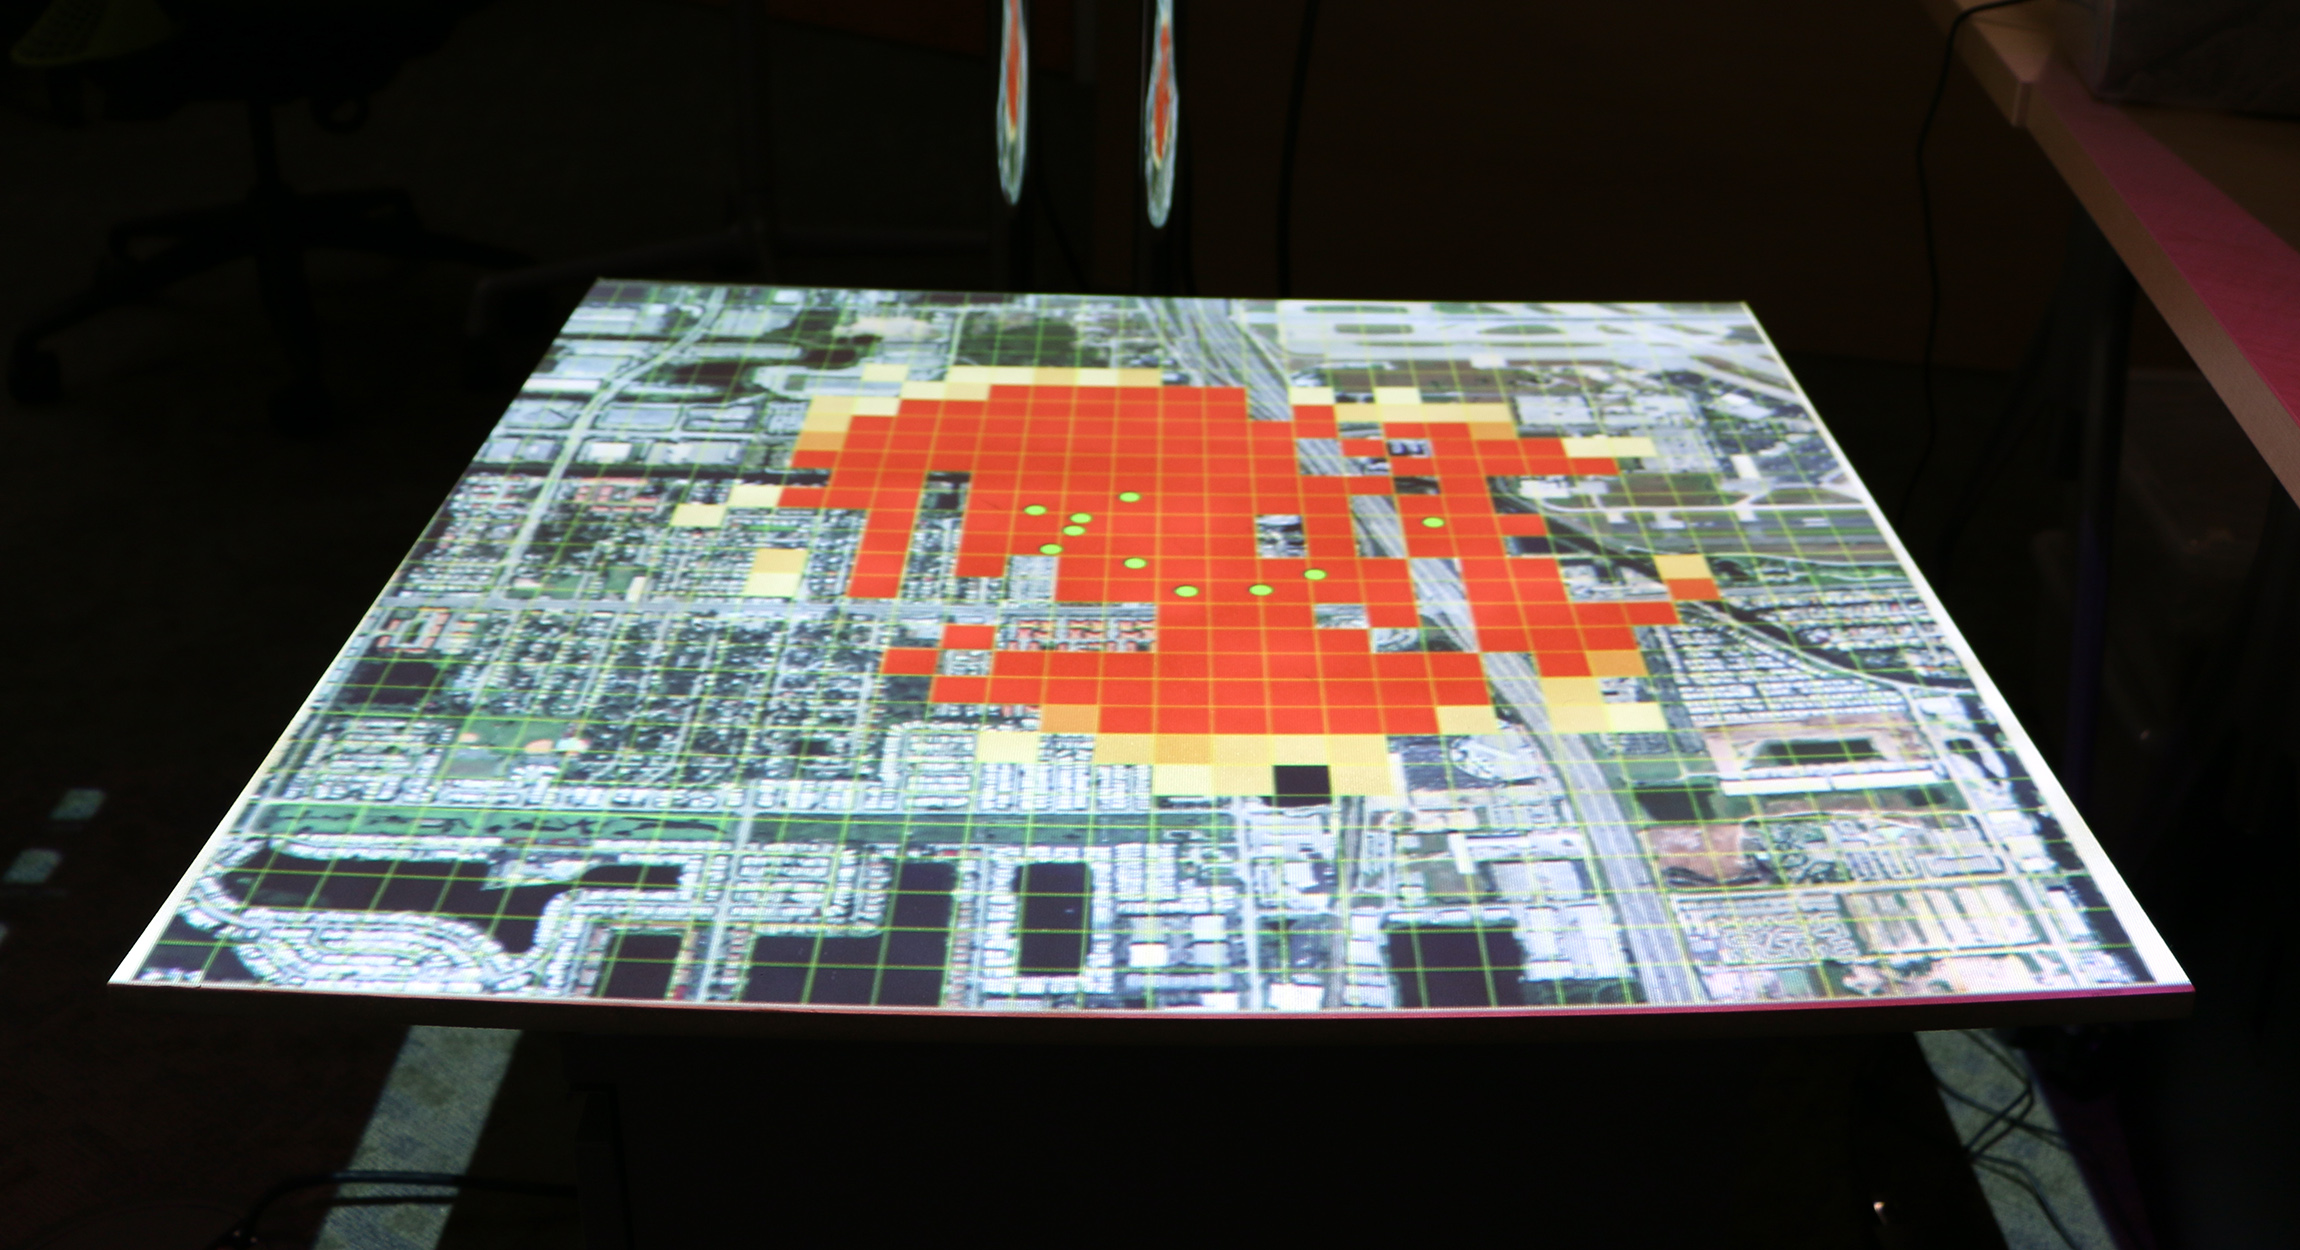
\includegraphics[width=0.3\textwidth]{images/termite_game_1.jpg}
		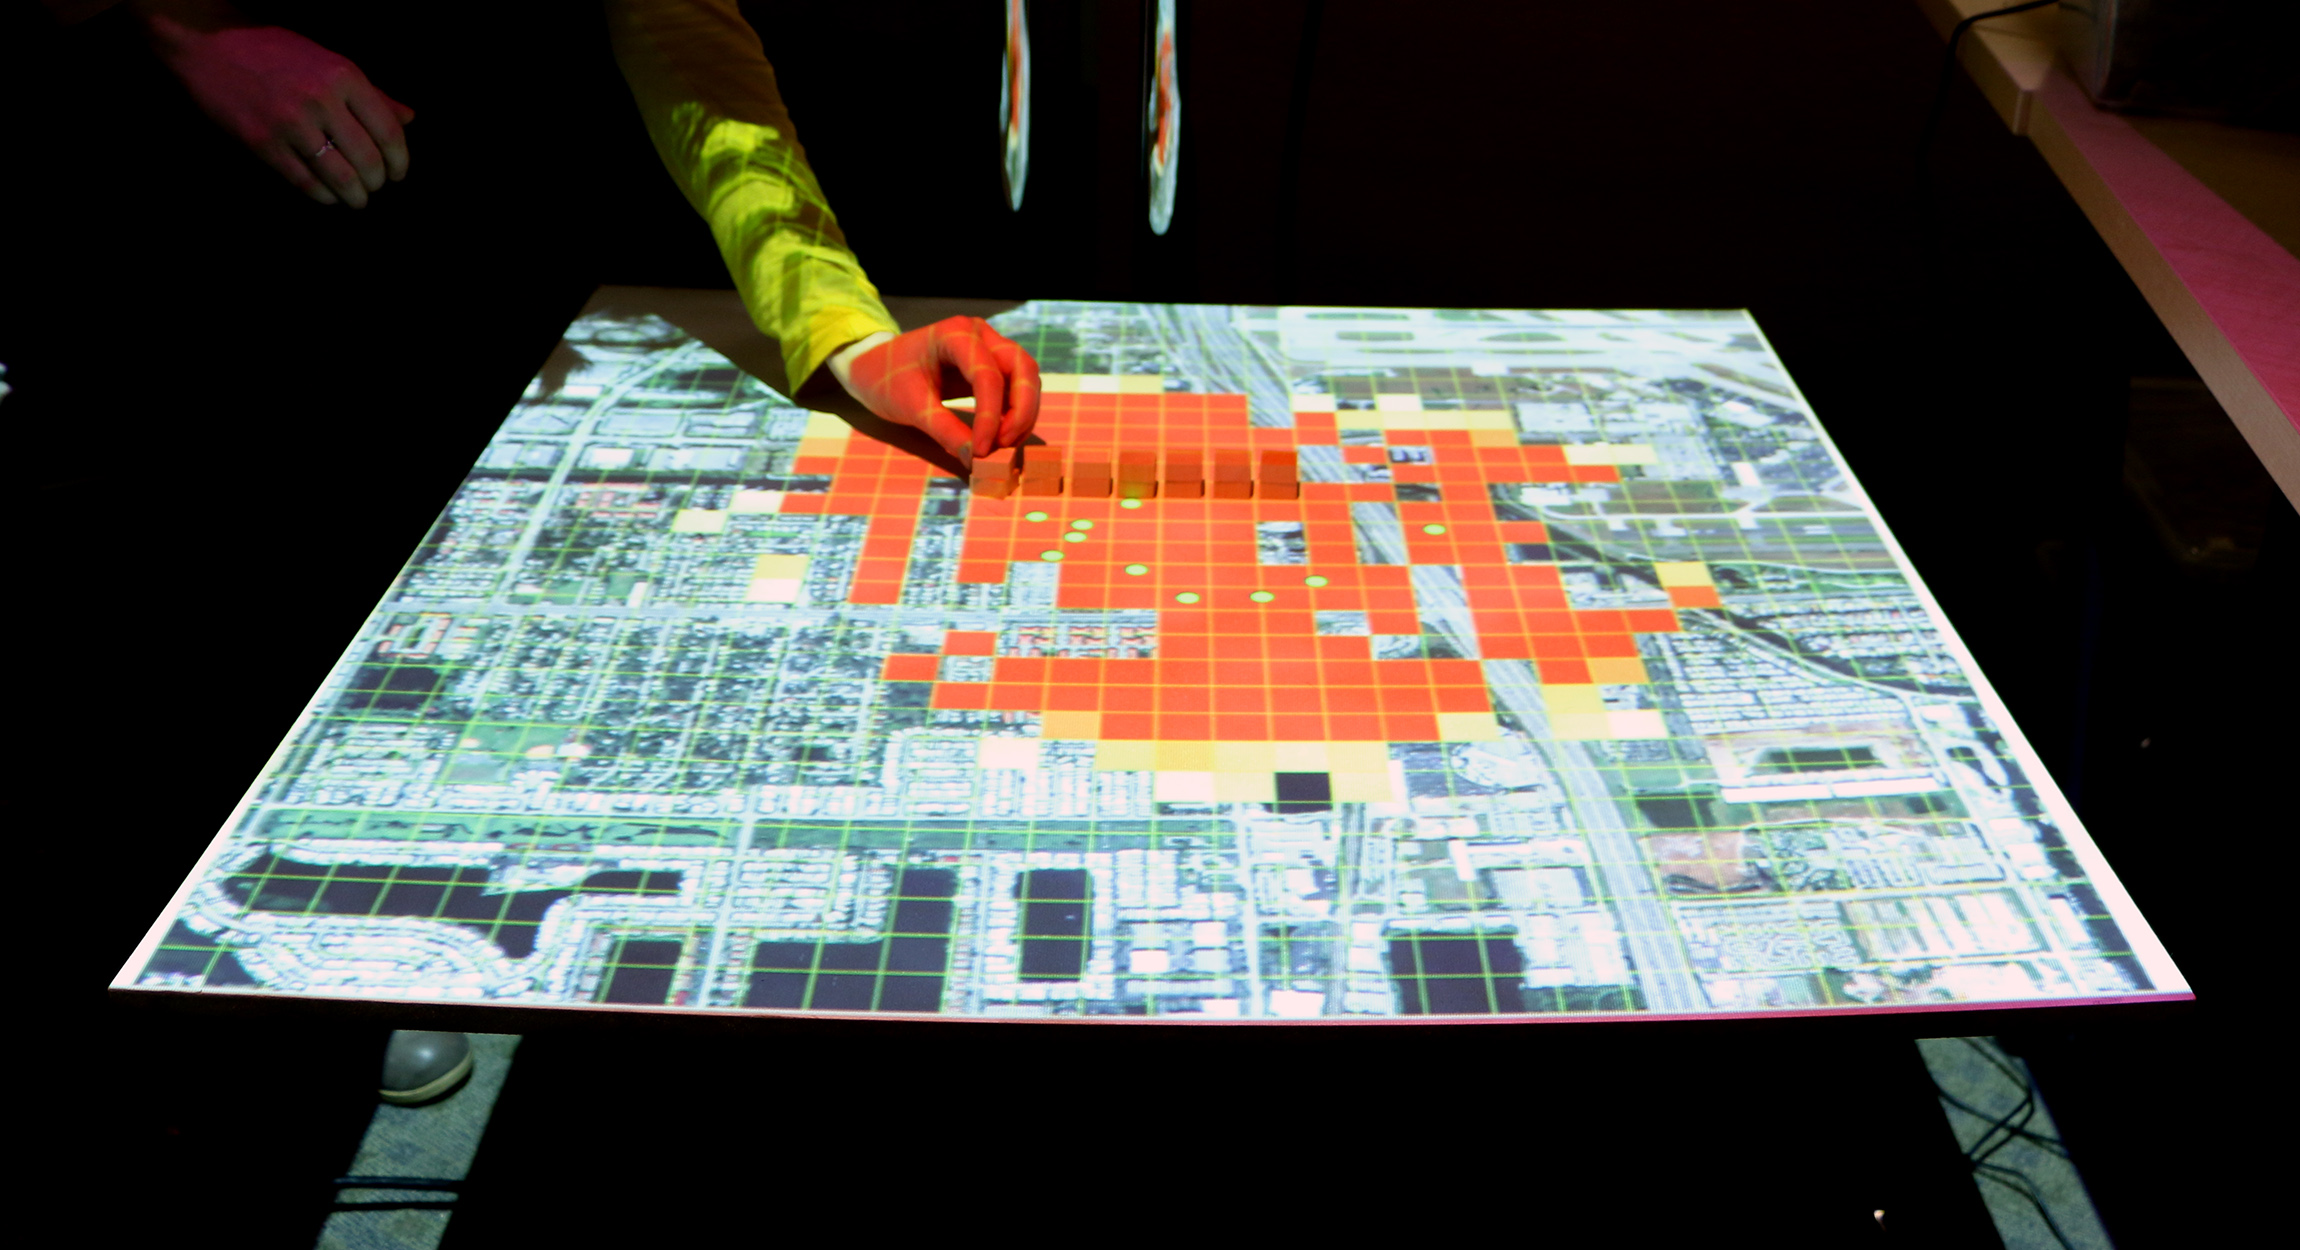
\includegraphics[width=0.3\textwidth]{images/termite_game_2.jpg}
		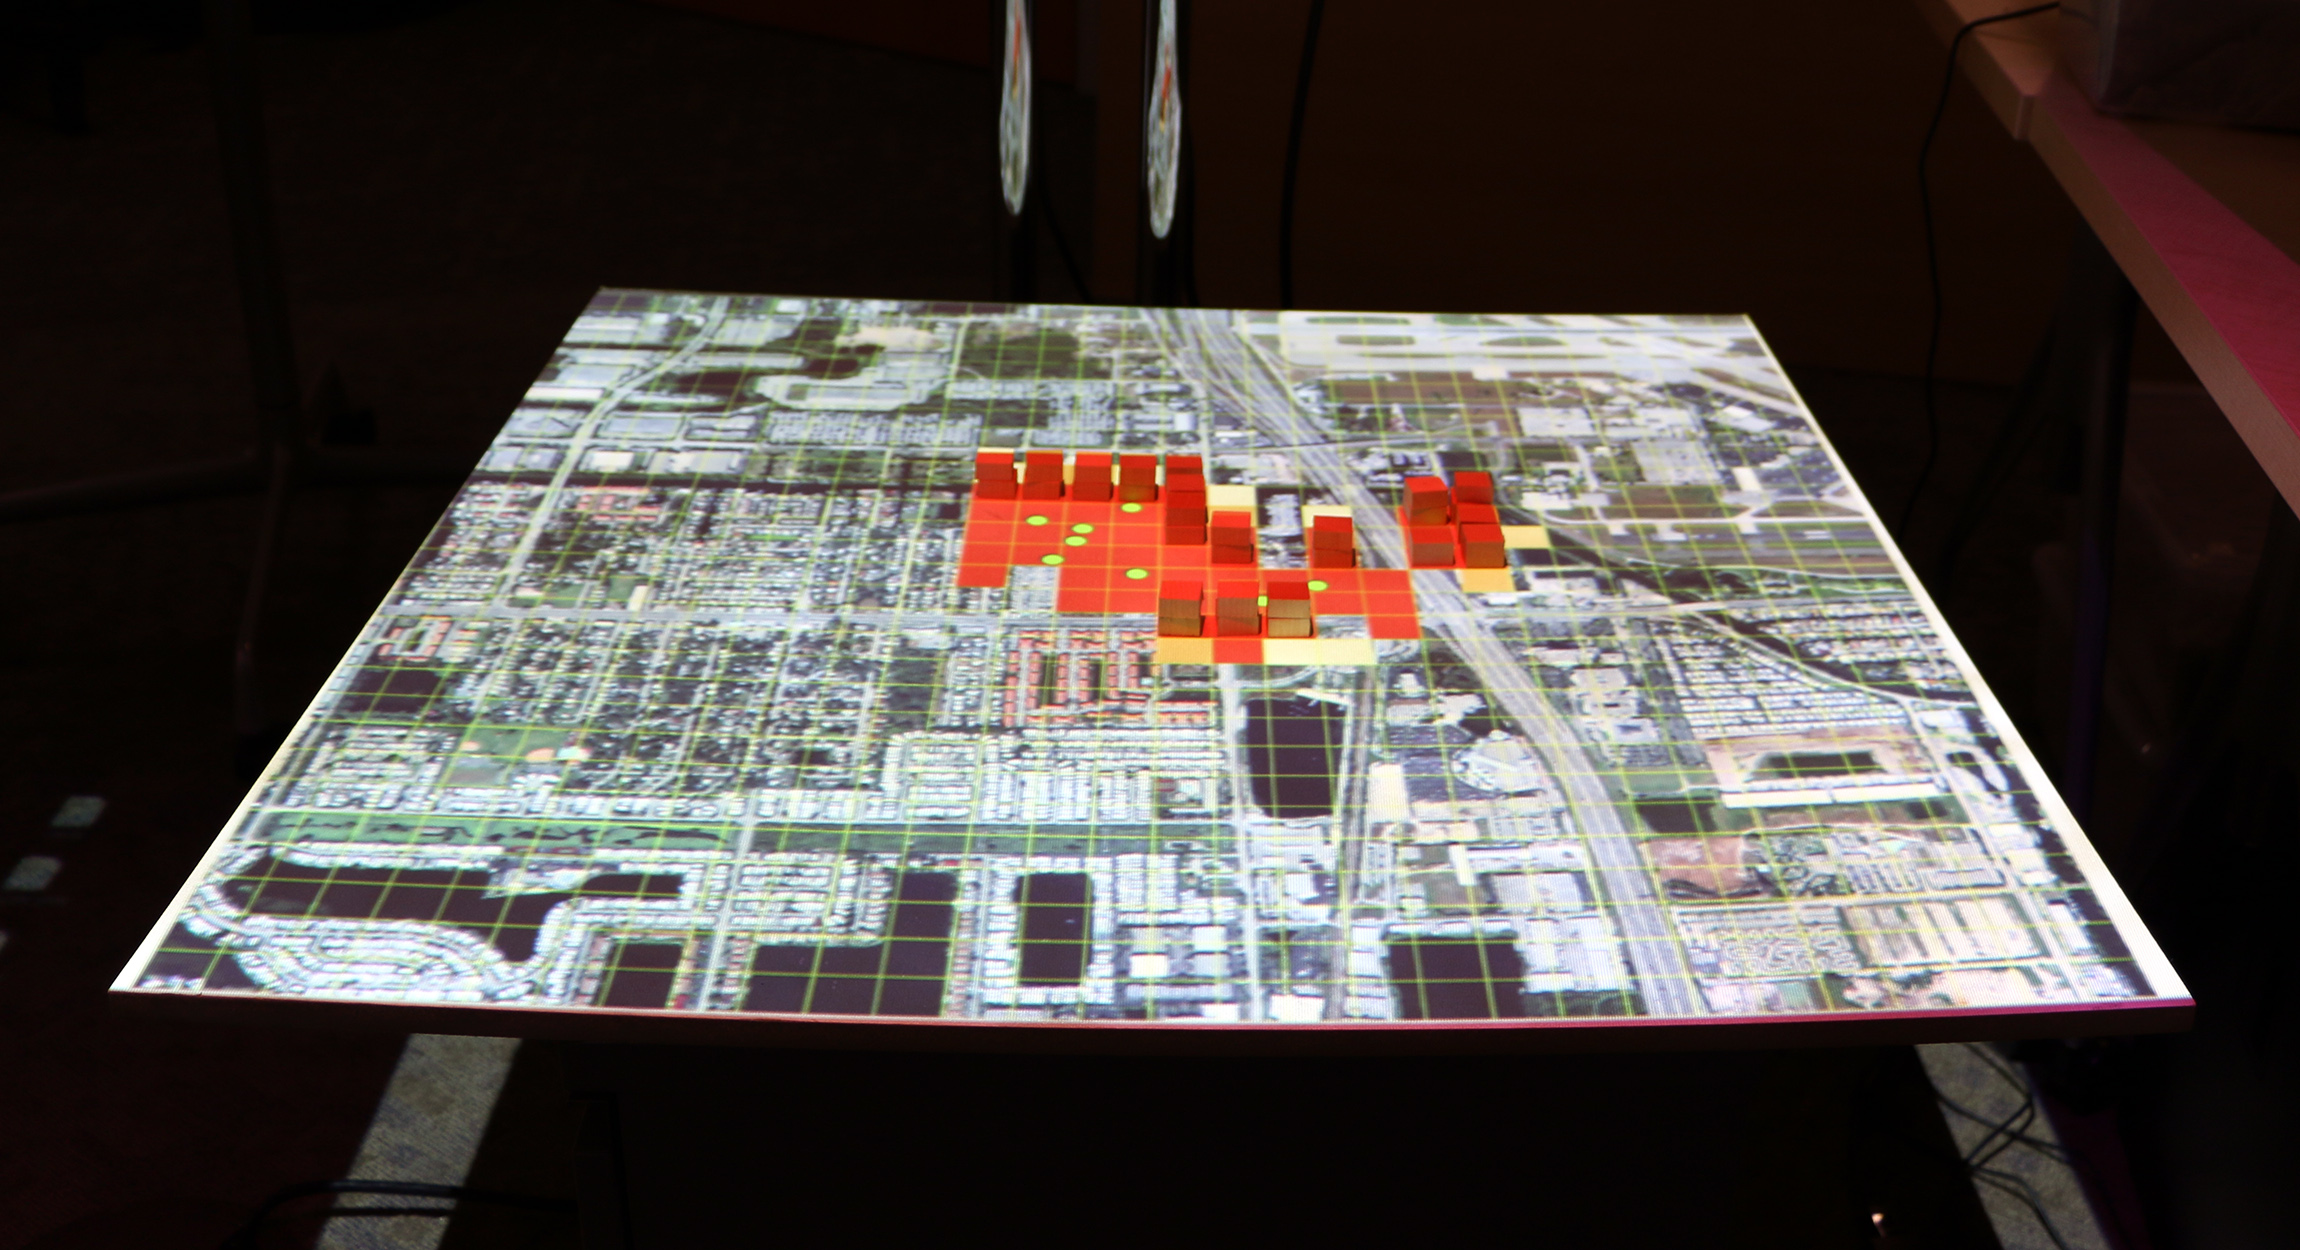
\includegraphics[width=0.3\textwidth]{images/termite_game_3.jpg}
	\caption{Managing the simulated spread of termites through a city with Tangible Landscape}
	\label{fig:termite_game}
\end{center}
\end{figure*}

\begin{figure*}[ht!]
\begin{center}
		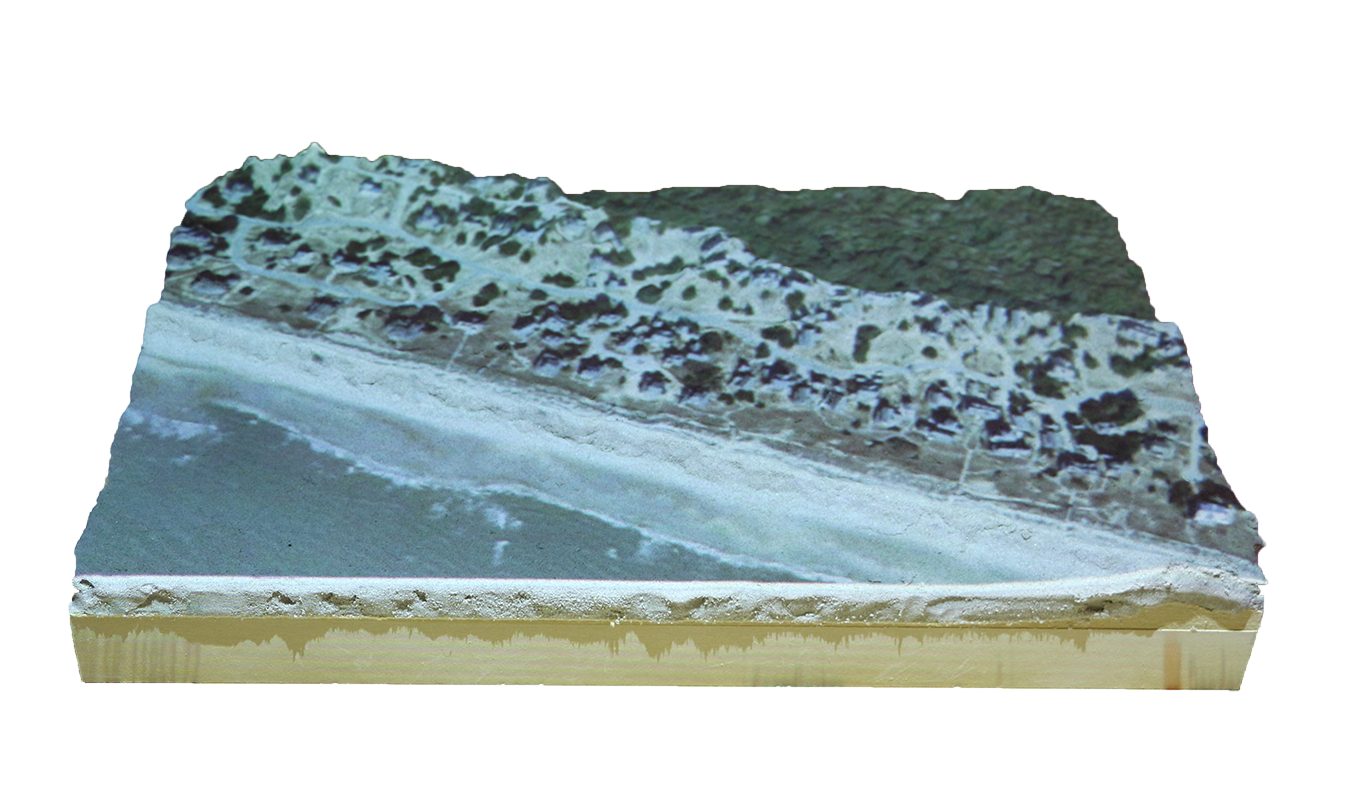
\includegraphics[width=0.3\textwidth]{images/tl_coastal_1s.png}
		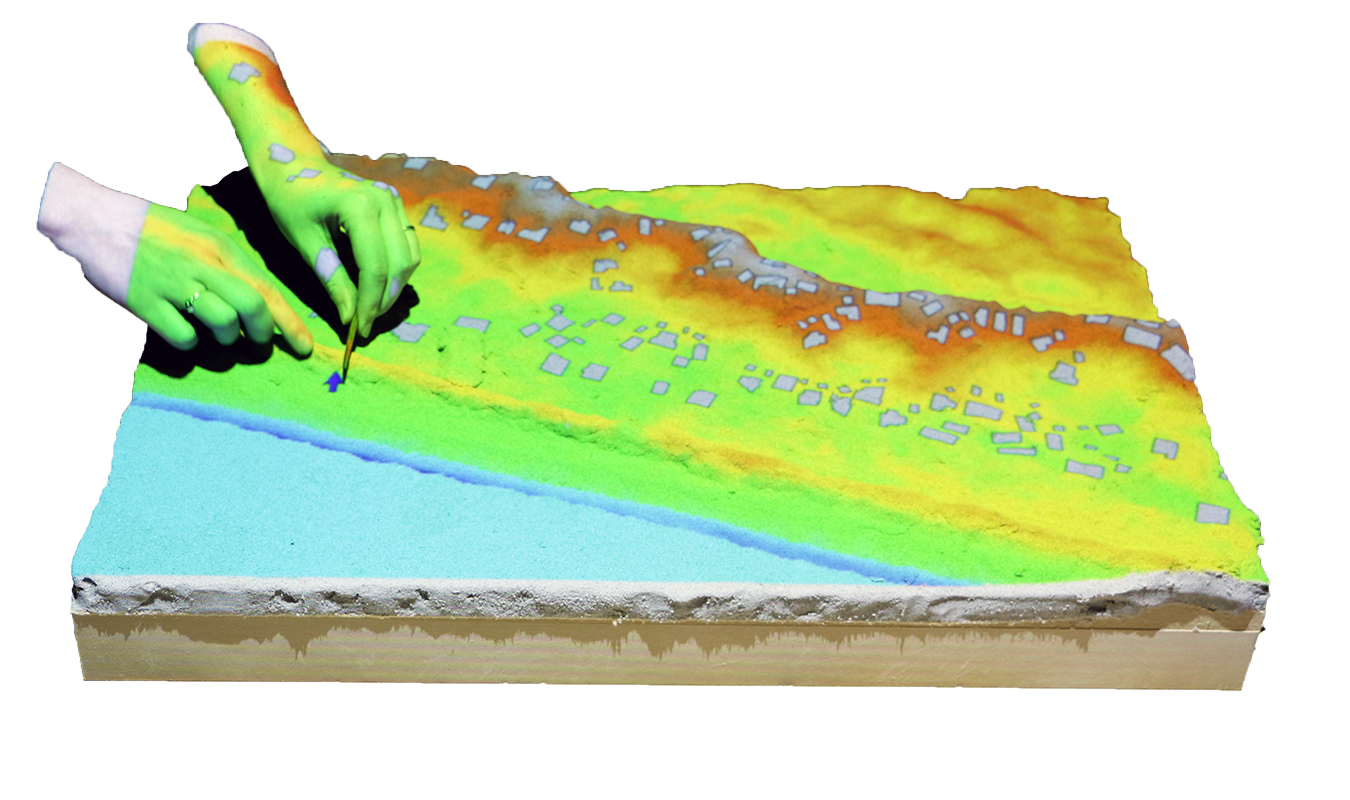
\includegraphics[width=0.3\textwidth]{images/tl_coastal_3s.png}
		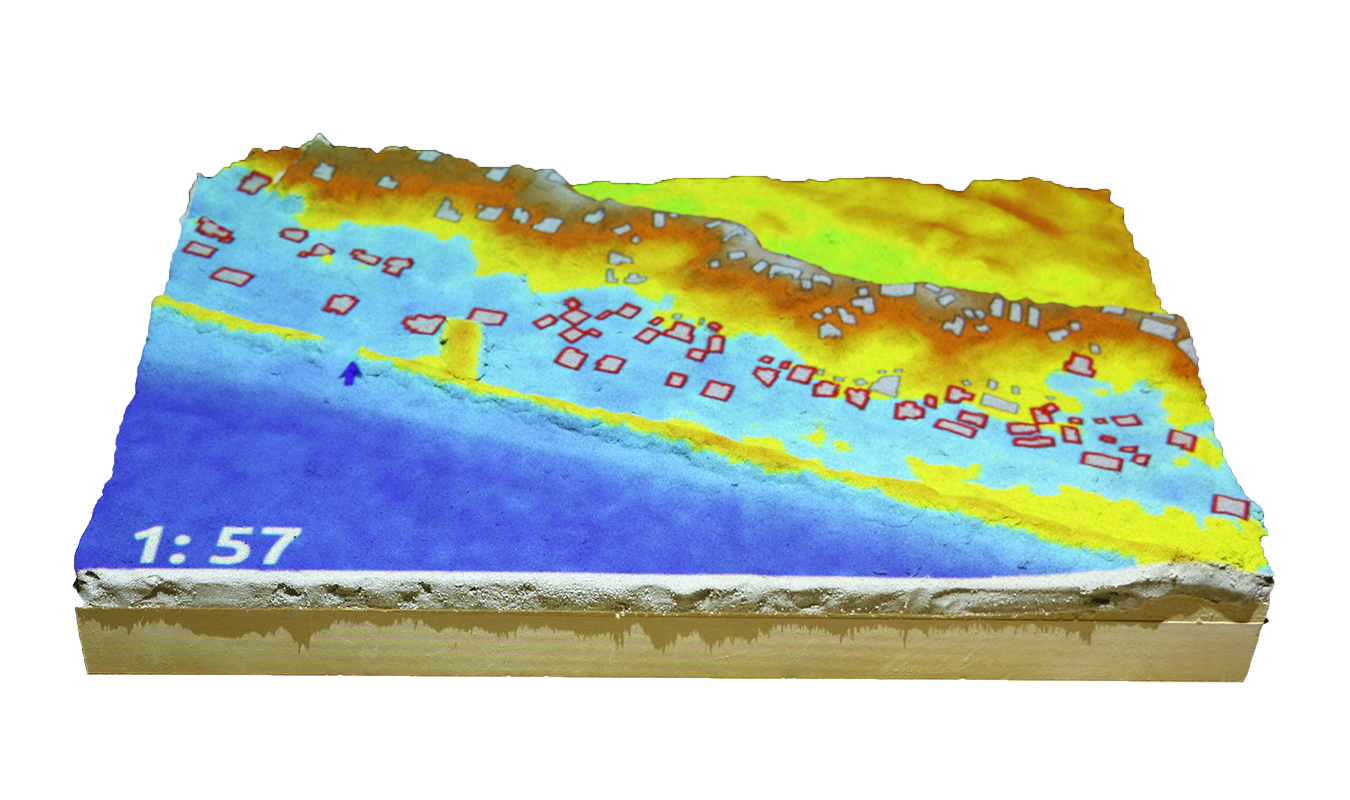
\includegraphics[width=0.3\textwidth]{images/tl_coastal_4s.png}
	\caption{...}
	\label{fig:coastal_game}
\end{center}
\end{figure*}

\section{Results}

\section{Discussion}


% How did the experiment address these research questions?

% DESIGN
% How can we design an effective tangible interface for GIS?
	% Experiment results and case study -> tested and informed design -> iterative process
		% describe realizing need for serious games
		% describe refinement of differencing

% COUPLING
% Can coupling a physical and digital model of topography improve spatial performance?

% ANALYTICS
% How do different geospatial analytics mediate users' spatial performance when using a tangible interface for GIS?






% Iterative design process
	% TLv2 w/ PCL + OpenKinect
	% New analyses for experiment
	
%\subsection{Design guidelines}
%\cite{Wilson2014}

\subsection{Open science}
% Call for collaboration with TL and experiment

\section{Future work}

% Time series analysis

% Vector flow fields and contour evolution

% Improved differencing analytic (faster with TLv2 w/ PCL + OpenKinect)
	% continual real-time mode

% Cognitive science
	% Cognitive, affective, motivational, and metacognitive processes

% TL remote computing and parallelization

% Real-time robotic fabrication
Figure~\ref{fig:system_schema_land} \ldots 

\begin{figure}%[h!]
\begin{center}
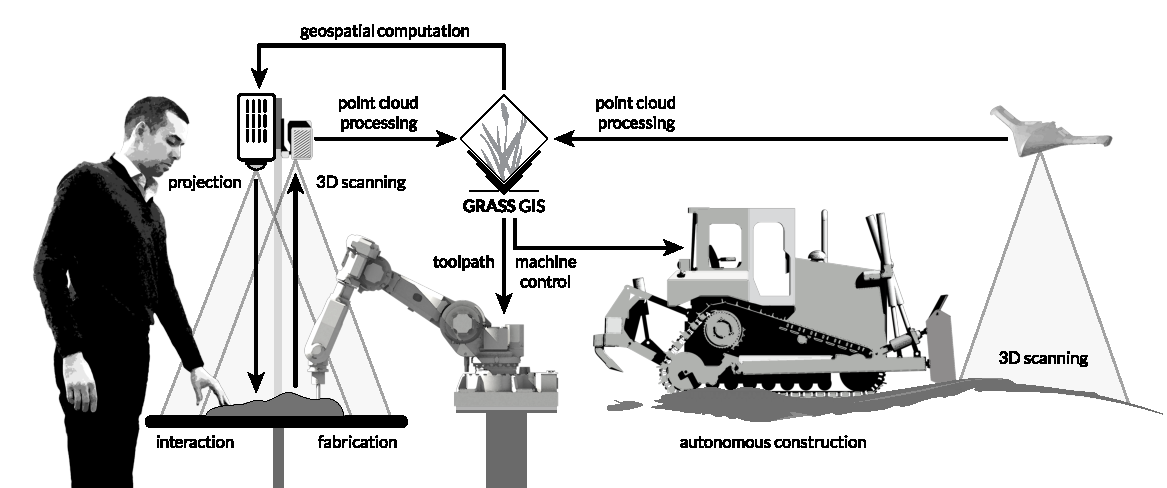
\includegraphics[width=\textwidth]{images/system_schema_land.pdf}
\caption{Tangible Landscape with robotic fabrication, robotic construction, and real-time field data}
\label{fig:system_schema_land}
\end{center}
\end{figure}

\section{Conclusion}

% Vision






%\section{...}
%% label
%\label{sec:examples}
%
%% Head 2
%\subsection{Head 2}
%
%% Head 3
%\subsubsection{Head 3}
%
%% Head 4
%\paragraph{Head 4}
%
%% quote
%\begin{quote}
%``\ldots".
%\end{quote}
%
%% itemize
%\begin{itemize}
%\item \ldots .
%\item \ldots .
%\item \ldots .
%\end{itemize}
%
%% footnote
%\ldots \footnote{...} 
%
%% enumerate
%\begin{enumerate}
%\item \ldots .
%\item \ldots . 
%\item \ldots .
%      \begin{enumerate}
%      \item \ldots .
%      \item \ldots .
%      \end{enumerate}
%\end{enumerate}
%
%% Enunciations
%\begin{definition}[...]...
%\end{definition}
%
%Table~\ref{tab:one}. 
%% Table
%\begin{table}%
%\tbl{...\label{tab:one}}{%
%\begin{tabular}{|l|l|}
%\hline
%...   & ...\\\hline
%...    & ...\\\hline
%\end{tabular}}
%\end{table}%

% Appendix
\appendix
\section*{APPENDIX}
\setcounter{section}{1}
In this appendix \ldots
\appendixhead{HARMON}

% Acknowledgments
\begin{acks}
\ldots
\end{acks}

% Bibliography
\bibliographystyle{ACM-Reference-Format-Journals}
\bibliography{tangible_topography.bib}

% History dates
%\received{}{}{}

% Electronic Appendix
\elecappendix

\medskip

\section{How to build Tangible Landscape}

\subsection{Hardware}
\begin{table}[hp!] \footnotesize \center
\caption{Hardware}
{\tabulinesep=1.2mm
\begin{tabu}{l l l}
\toprule
Type & Product & Cost\\
\midrule
Computer & System 76 Oryx Pro & \$1500\\
Projector & Optoma ML750 WXGA 700 DLP LED & \$500\\
3D sensor & Xbox One Kinect & \$100\\
& Kinect Adapter for Windows & \$50\\
Stand & Avenger 40-Inch C-Stand with Grip Kit & \$200\\
& Avenger 40-Inch C-Stand with Grip Kit & \$200\\
& Avenger F800 3-Inch Baby Wall Plate & \$10\\
& Avenger F800 3-Inch Baby Wall Plate & \$10\\
Peripherals & HDMI cable & \$10\\
& Extension cord & \$10\\
Modeling media & Waba Fun Kinetic Sand 11 Lbs & \$50\\
\bottomrule
\end{tabu}}
\label{table:hardware} 
\end{table}

\subsection{Setup}


\section{Setting up the experiment}






%\subsection{Data sources}
%\begin{table}[hp!] \footnotesize \center
%\caption{Data sources}
%{\tabulinesep=1.2mm
%\begin{tabu}{l l l}
%\toprule
%Data type & Data source & Link\\
%\midrule
%Lidar & United States Interagency Elevation Inventory & http://coast.noaa.gov/inventory/\\
%& Earth Explorer & http://earthexplorer.usgs.gov/\\
%& Digital Coast & http://coast.noaa.gov/dataviewer/\\
%& Open Topography & http://www.opentopography.org/\\
%Digital Elevation Models & National Elevation Dataset & http://viewer.nationalmap.gov/viewer/\\
%Orthoimagery & USGS EROS Orthoimagery WMS & http://raster.nationalmap.gov/\\
%\bottomrule
%\end{tabu}}
%\label{table:data_sources} 
%\end{table}
























\end{document}



